%
% A header that lets you compile a chapter by itself, or inside a larger document.
% Adapted from stackoverflow.com/questions/3655454/conditional-import-in-latex
%
%
%Use \inbpdocument and \outbpdocument in your individual files, in place of \begin{document} and \end{document}. In your main file, put in a \def \ismaindoc {} before including or importing anything.
%
% David Duvenaud
% June 2011
% 
% ======================================
%
%


\ifx\ismaindoc\undefined
	\newcommand{\inbpdocument}{
		\def \ismaindoc {}
		% Use this header if we are compiling by ourselves.
		\documentclass[a4paper,11pt,authoryear,index]{common/PhDThesisPSnPDF}
		
%\usepackage{draftwatermark}
%\SetWatermarkLightness{0.95}

% ******************************************************************************
% ****************************** Custom Margin *********************************

% Add `custommargin' in the document class options to use this section
% Set {innerside margin / outerside margin / topmargin / bottom margin}  and
% other page dimensions

\ifsetMargin
\else
    \RequirePackage[left=37mm,right=30mm,top=35mm,bottom=30mm]{geometry}
    \setFancyHdr % To apply fancy header after geometry package is loaded
\fi


%\chead{Unfinished draft}
%\cfoot{\texttt{Unfinished draft - compiled on \today{} at \currenttime}}

% *****************************************************************************
% ******************* Fonts (like different typewriter fonts etc.)*************

% Add `customfont' in the document class option to use this section

\ifsetFont
\else
    % Set your custom font here and use `customfont' in options. Leave empty to
    % load computer modern font (default LaTeX font).  

    \RequirePackage{libertine} 
\fi

% *****************************************************************************
% *************************** Bibliography  and References ********************

%\usepackage{cleveref} %Referencing without need to explicitly state fig /table

% Add `custombib' in the document class option to use this section
\ifsetBib % True, Bibliography option is chosen in class options
\else % If custom bibliography style chosen then load bibstyle here

   \RequirePackage[square, sort, numbers, authoryear]{natbib} % CustomBib

% If you would like to use biblatex for your reference management, as opposed to the default `natbibpackage` pass the option `custombib` in the document class. Comment out the previous line to make sure you don't load the natbib package. Uncomment the following lines and specify the location of references.bib file

% \RequirePackage[backend=biber, style=numeric-comp, citestyle=numeric, sorting=nty, natbib=true]{biblatex}
% \bibliography{References/references} %Location of references.bib only for biblatex

\fi


% changes the default name `Bibliography` -> `References'
\renewcommand{\bibname}{References}


% *****************************************************************************
% *************** Changing the Visual Style of Chapter Headings ***************
% Uncomment the section below. Requires titlesec package.

%\RequirePackage{titlesec}
%\newcommand{\PreContentTitleFormat}{\titleformat{\chapter}[display]{\scshape\Large}
%{\Large\filleft{\chaptertitlename} \Huge\thechapter}
%{1ex}{}
%[\vspace{1ex}\titlerule]}
%\newcommand{\ContentTitleFormat}{\titleformat{\chapter}[display]{\scshape\huge}
%{\Large\filleft{\chaptertitlename} \Huge\thechapter}{1ex}
%{\titlerule\vspace{1ex}\filright}
%[\vspace{1ex}\titlerule]}
%\newcommand{\PostContentTitleFormat}{\PreContentTitleFormat}
%\PreContentTitleFormat


% *****************************************************************************
% **************************** Custom Packages ********************************
% *****************************************************************************


% ************************* Algorithms and Pseudocode **************************

%\usepackage{algpseudocode} 


% ********************Captions and Hyperreferencing / URL **********************

% Captions: This makes captions of figures use a boldfaced small font. 
%\RequirePackage[small,bf]{caption}

\RequirePackage[labelsep=space,tableposition=top]{caption} 
%\renewcommand{\figurename}{Figure} %to support older versions of captions.sty
\captionsetup{labelsep = colon,belowskip=12pt,aboveskip=4pt}

% ************************ Formatting / Footnote *******************************

%\usepackage[perpage]{footmisc} %Range of footnote options 


% ****************************** Line Numbers **********************************

%\RequirePackage{lineno}
%\linenumbers

% ************************** Graphics and figures *****************************

%\usepackage{rotating}
%\usepackage{wrapfig}
%\usepackage{float}
\usepackage{subfig} %note: subfig must be included after the `caption` package. 


% ********************************* Table **************************************

%\usepackage{longtable}
%\usepackage{multicol}
%\usepackage{multirow}
%\usepackage{tabularx}


% ***************************** Math and SI Units ******************************

\usepackage{amsfonts}
\usepackage{amsmath}
\usepackage{amssymb}
%\usepackage{siunitx} % use this package module for SI units


% ******************************************************************************
% ************************* User Defined Commands ******************************
% ******************************************************************************

% *********** To change the name of Table of Contents / LOF and LOT ************

%\renewcommand{\contentsname}{My Table of Contents}
%\renewcommand{\listfigurename}{List of figures}
%\renewcommand{\listtablename}{List of tables}


% ********************** TOC depth and numbering depth *************************

\setcounter{secnumdepth}{2}
\setcounter{tocdepth}{2}

% ******************************* Nomenclature *********************************

% To change the name of the Nomenclature section, uncomment the following line

%\renewcommand{\nomname}{Symbols}


% ********************************* Appendix ***********************************

% The default value of both \appendixtocname and \appendixpagename is `Appendices'. These names can all be changed via: 

%\renewcommand{\appendixtocname}{List of appendices}
%\renewcommand{\appendixname}{Appndx}

		% All my custom preamble stuff.  Shouldn't overlap with anything in official-preamble




% Paths to figure and table directories.
\newcommand{\symmetryfigsdir}{figures/symmetries}
\newcommand{\topologyfiguresdir}{figures/topology}
\newcommand{\infinitefiguresdir}{figures/infinite}
\newcommand{\grammarfiguresdir}{figures/grammar}
\newcommand{\introfigsdir}{figures/intro}
\newcommand{\gplvmfiguresdir}{figures/gplvm}
\newcommand{\warpedfiguresdir}{figures/warped-mixtures}
\newcommand{\deeplimitsfiguresdir}{figures/deep-limits}
\newcommand{\quadraturefigsdir}{figures/quadrature}
\newcommand{\additivefigsdir}{figures/additive}
\newcommand{\decompfigsdir}{figures/decomp}
\newcommand{\examplefigsdir}{figures/worked-example}

\usepackage{bm}  % for warped mixtures - is this necessary?
\usepackage{booktabs}
\usepackage{tabularx}
\usepackage{multirow}
\usepackage{datetime}
\renewcommand{\tabularxcolumn}[1]{>{\arraybackslash}m{#1}}
\usepackage{relsize}
\usepackage{graphicx}
\usepackage{amsmath,amssymb,textcomp}
\usepackage{nicefrac}
\usepackage{amsthm}
\usepackage{tikz}
\usetikzlibrary{arrows}
\usetikzlibrary{calc}
\usepackage{nth}
\usepackage{rotating}
\usepackage{array}
\usepackage{fp}
\usepackage{cleveref}   % Note: this package sometimes causes the page counter to reset.
\crefname{equation}{equation}{equations}
\crefname{figure}{figure}{figures}
%\usepackage{common/sectsty}

% Controls capitalization of all headers
%\usepackage{stringstrings}
%\usepackage[explicit]{titlesec}
%\newcommand\SentenceCase[1]{%
%  \caselower[e]{#1}%
%  \capitalize[q]{\thestring}%
%}
%\titleformat{\section}
%  {\normalfont\Large\bfseries}{\thesection}{1em}{\SentenceCase{#1}\thestring}


%\titleformat{\section} % The normal, unstarred version
%    {\Large\bfseries}{}{2ex}
%    {\thesection. \MakeSentenceCase{#1}}

%\titleformat{name=\section,numberless} % The starred version; note the `numberless` key
%    {\Large\bfseries}{}{2ex}
%    {\MakeSentenceCase{#1}}

\usepackage[hyperpageref]{backref}
% Setup to show (pages 4 and 9) sort of thing in the bibliography - DD
%\def\foo{\hspace{\fill}\mbox{}\linebreak[0]\hspace*{\fill}}
%\def\foo{\parbox{3cm}{\hfill}
%\def\foo{\parbox{3cm}{\hfill}
%\newcommand\foo[1]{{\raggedleft{\hfill{\mbox{\hfill{#1}}}}}}
\newcommand{\comfyfill}[1]{% = Thorsten Donig's \signed
  \unskip\hspace*{0.1em plus 1fill}
  \nolinebreak[3]%
  \hspace*{\fill}\mbox{#1}
  \parfillskip0pt\par
}
\newcommand\foo[1]{{\comfyfill{\mbox{#1}}}}
%\newcommand\foo[1]{{\mbox{#1}}}
\renewcommand*{\backref}[1]{}
\renewcommand*{\backrefalt}[4]{%
\ifcase #1 %
%
\or
\foo{(page #2)}%
\else
\foo{(pages #2)}%
\fi
}

\usepackage{stringstrings}

%\newcommand{\headercase}{\
%\DeclareFieldFormat{titlecase}{\MakeSentenceCase{#1}}


%% For submission, make all render blank.
%%%%%%%%%%%%%%%%%%%%%%%%%%%%%%%%%%%%%%%%%%%%%%%%%%%%%%%%%%
%%%% EDITING HELPER FUNCTIONS  %%%%%%%%%%%%%%%%%%%%%%%%%%%
%%%%%%%%%%%%%%%%%%%%%%%%%%%%%%%%%%%%%%%%%%%%%%%%%%%%%%%%%%

%% NA: needs attention (rough writing whose correctness needs to be verified)
%% TBD: instructions for how to fix a gap ("Describe the propagation by ...")
%% PROBLEM: bug or missing crucial bit 

%% use \fXXX versions of these macros to put additional explanation into a footnote.  
%% The idea is that we don't want to interrupt the flow of the paper or make it 
%% impossible to read because there are a bunch of comments.

%% NA's (and TBDs, those less crucially) should be written so 
%% that they flow with the text.

\definecolor{WowColor}{rgb}{.75,0,.75}
\definecolor{SubtleColor}{rgb}{0,0,.50}

% inline
\newcommand{\NA}[1]{\textcolor{SubtleColor}{ {\tiny \bf ($\star$)} #1}}
\newcommand{\LATER}[1]{\textcolor{SubtleColor}{ {\tiny \bf ($\dagger$)} #1}}
\newcommand{\TBD}[1]{\textcolor{SubtleColor}{ {\tiny \bf (!)} #1}}
\newcommand{\PROBLEM}[1]{\textcolor{WowColor}{ {\bf (!!)} {\bf #1}}}

% as margin notes

\newcounter{margincounter}
\newcommand{\displaycounter}{{\arabic{margincounter}}}
\newcommand{\incdisplaycounter}{{\stepcounter{margincounter}\arabic{margincounter}}}

\newcommand{\fTBD}[1]{\textcolor{SubtleColor}{$\,^{(\incdisplaycounter)}$}\marginpar{\tiny\textcolor{SubtleColor}{ {\tiny $(\displaycounter)$} #1}}}

\newcommand{\fPROBLEM}[1]{\textcolor{WowColor}{$\,^{((\incdisplaycounter))}$}\marginpar{\tiny\textcolor{WowColor}{ {\bf $\mathbf{((\displaycounter))}$} {\bf #1}}}}

\newcommand{\fLATER}[1]{\textcolor{SubtleColor}{$\,^{(\incdisplaycounter\dagger)}$}\marginpar{\tiny\textcolor{SubtleColor}{ {\tiny $(\displaycounter\dagger)$} #1}}}

%\renewcommand{\LATER}[1]{}
%\renewcommand{\fLATER}[1]{}
%\renewcommand{\TBD}[1]{}
%\renewcommand{\fTBD}[1]{}
%\renewcommand{\PROBLEM}[1]{}
%\renewcommand{\fPROBLEM}[1]{}
%\renewcommand{\NA}[1]{}


% HUMBLE WORDS: shown slightly smaller when in normal text
% Thanks to Christian Steinruecken!

% HUMBLE WORDS: shown slightly smaller when in normal text
% Christian Steinruecken
%
\makeatletter%
%\def\@humbleformat#1{{\fontsize{}{1em}\selectfont #1}}
%\def\@humbleformat#1{\textsmaller{#1}}%
\newlength{\nonHumbleHeight}
\def\@humbleformat#1{{\settoheight{\nonHumbleHeight}{#1}\resizebox{!}{0.94\nonHumbleHeight}{#1}}}%
\def\@idxhumbleformat#1{{\relscale{0.95}{#1}}}%
%\def\@humbleformat#1{{#1}}%
\def\declareHumble#1#2{%
  \expandafter\def\csname #1\endcsname{\@humbleformat{#2}}%
  \expandafter\def\csname s#1\endcsname{{#2}}%
  \expandafter\def\csname idx#1\endcsname{{\@idxhumbleformat{#2}}}%
}%
\def\humble#1{\@humbleformat{#1}}%
\def\idxhumble#1{\@idxhumbleformat{#1}}%
\makeatother%

% Convenient indexing for humble abbreviations
\def\humbleindex#1#2{\index{#1@\idxhumble{#1}}}



% TODO: Clean up duplicates
\declareHumble{ANOVA}{ANOVA}
\declareHumble{ARD}{ARD}
\declareHumble{BIC}{BIC}
\declareHumble{BMC}{BMC}
\declareHumble{bq}{BQ}
\declareHumble{CRP}{CRP}
\declareHumble{dirpro}{DP}
\declareHumble{HDMR}{HDMR}
\declareHumble{GAM}{GAM}
\declareHumble{GEM}{GEM}
\declareHumble{GMM}{GMM}
\declareHumble{gplvm}{GP-LVM}
\declareHumble{gpml}{GPML}
\declareHumble{GPML}{GPML}
\declareHumble{gprn}{GPRN}
\declareHumble{gpt}{GP}
\declareHumble{gp}{GP}
\declareHumble{HKL}{HKL}
\declareHumble{HMC}{HMC}
\declareHumble{ibp}{IBP}
\declareHumble{iGMM}{iGMM}
\declareHumble{iwmm}{iWMM}
\declareHumble{kCP}{CP}
\declareHumble{kCW}{CW}
\declareHumble{kC}{C}
\declareHumble{KDE}{KDE}
\declareHumble{kLin}{Lin}
\declareHumble{KPCA}{KPCA}
\declareHumble{kPer}{Per}
\declareHumble{kPerGen}{ZMPer}
\declareHumble{kRQ}{RQ}
\declareHumble{kSE}{SE}
\declareHumble{kWN}{WN}
\declareHumble{Lin}{Lin}
\declareHumble{LBFGS}{L-BFGS}
\declareHumble{LIBSVM}{LIBSVM}
\declareHumble{MAP}{MAP}
\declareHumble{mcmc}{MCMC}
\declareHumble{MKL}{MKL}
\declareHumble{MLP}{MLP}
\declareHumble{MNIST}{MNIST}
\declareHumble{MSE}{MSE}
\declareHumble{OU}{OU}
\declareHumble{Per}{Per}
\declareHumble{RBF}{RBF}
\declareHumble{RMSE}{RMSE}
\declareHumble{RQ}{RQ}
\declareHumble{SBQ}{SBQ}
\declareHumble{seard}{SE-ARD}
\declareHumble{sefull}{SE-\textnormal{full}}
\declareHumble{SEGP}{SE-GP}
\declareHumble{SE}{SE}
\declareHumble{SNR}{SNR}
\declareHumble{SSANOVA}{SS-ANOVA}
\declareHumble{SVM}{SVM}
\declareHumble{UCI}{UCI}
\declareHumble{UMIST}{UMIST}
\declareHumble{vbgplvm}{VB GP-LVM}

\newcommand{\kSig}{\boldsymbol\sigma}

\def\subexpr{{\cal S}}
\def\baseker{{\cal B}}
\def\numWinners{k}

\def\ie{i.e.\ }
\def\eg{e.g.\ }
\def\etc{etc.\ }
\let\oldemptyset\emptyset
%\let\emptyset 0




% Unify notation between neural-net land and GP-land.
\newcommand{\hphi}{h}
\newcommand{\hPhi}{\vh}
\newcommand{\walpha}{w}
\newcommand{\wboldalpha}{\bw}
\newcommand{\wcapalpha}{\vW}
\newcommand{\lengthscale}{w}

\newcommand{\layerindex}{\ell}



\newcommand{\gpdrawbox}[1]{
\setlength\fboxsep{0pt}
\hspace{-0.15in} 
\fbox{
\includegraphics[width=0.464\columnwidth]{\deeplimitsfiguresdir/deep_draws/deep_gp_sample_layer_#1}
}}



\newcommand{\procedurename}{ABCD}
\newcommand{\genText}[1]{{\sf #1}}



\newcommand{\asdf}{$^{\textnormal{th}}$}

\newcommand{\binarysum}{\sum_{\bf{x} \in \{0,1\}^D}}
\newcommand{\expect}{\mathbb{E}}
\newcommand{\expectargs}[2]{\mathbb{E}_{#1} \left[ {#2} \right]}
\newcommand{\var}{\mathbb{V}}
\newcommand{\varianceargs}[2]{\mathbb{V}_{#1} \left[ {#2} \right]}
\newcommand{\cov}{\operatorname{cov}}
\newcommand{\Cov}{\operatorname{Cov}}
\newcommand{\covargs}[2]{\Cov \left[ {#1}, {#2} \right]}
\newcommand{\variance}{\mathbb{V}}
\newcommand{\vecop}[1]{\operatorname{vec} \left( {#1} \right)}

\newcommand{\covarianceargs}[2]{\Cov_{#1} \left[ {#2} \right]}
\newcommand{\colvec}[2]{\left[ \begin{array}{c} {#1} \\ {#2} \end{array} \right]}
\newcommand{\tbtmat}[4]{\left[ \begin{array}{cc} {#1} & {#2} \\ {#3} & {#4} \end{array} \right]}

\newcommand{\acro}[1]{{\humble{#1}}}
%\newcommand{\vect}[1]{\boldsymbol{#1}}
\newcommand{\vect}[1]{{\bf{#1}}}
\newcommand{\mat}[1]{\mathbf{#1}}
\newcommand{\pderiv}[2]{\frac{\partial #1}{\partial #2}}
\newcommand{\npderiv}[2]{\nicefrac{\partial #1}{\partial #2}}

\newcommand{\pha}{^{\phantom{:}}}

\newcommand{\argmin}{\operatornamewithlimits{argmin}}
\newcommand{\argmax}{\operatornamewithlimits{argmax}}

% The following designed for probabilities with long arguments

\newcommand{\Prob}[2]{P\!\left(\,#1\;\middle\vert\;#2\,\right)}
\newcommand{\ProbF}[3]{P\!\left(\,#1\!=\!#2\;\middle\vert\;#3\,\right)}
\newcommand{\p}[2]{p\!\left(#1\middle\vert#2\right)}
\newcommand{\po}[1]{p\!\left(#1\right)}
\newcommand{\pF}[3]{p\!\left(\,#1\!=\!#2\;\middle\vert\;#3\,\right)} 
\newcommand{\mean}[2]{{m}\!\left(#1\middle\vert#2\right)}



\newcommand{\valpha}{\boldsymbol{\alpha}}
\newcommand{\va}{\vect{a}}
\newcommand{\vA}{\vect{A}}
\newcommand{\vB}{\mat{B}}
\newcommand{\vb}{\vect{b}}
\newcommand{\vC}{\mat{C}}
\newcommand{\vc}{\vect{c}}
\newcommand{\vecf}{\boldsymbol{f}}
\newcommand{\vell}{\vect{\ell}}
\newcommand{\vepsilon}{\boldsymbol{\epsilon}}
\newcommand{\veps}{\boldsymbol{\epsilon}}
\newcommand{\ve}{\boldsymbol{\epsilon}}
\newcommand{\vf}{\vecf}
\newcommand{\vg}{\vect{g}}
\newcommand{\vh}{\vect{h}}
\newcommand{\vI}{\mat{I}}
\newcommand{\vK}{\mat{K}}
\newcommand{\vk}{\vect{k}}
\newcommand{\vL}{\mat{L}}
\newcommand{\vl}{\vect{l}}
\newcommand{\vmu}{{\boldsymbol{\mu}}}
\newcommand{\vone}{\vect{1}}
\newcommand{\vphi}{{\boldsymbol{\phi}}}
\newcommand{\vpi}{{\boldsymbol{\pi}}}
\newcommand{\vq}{\vect{q}}
\newcommand{\vR}{\mat{R}}
\newcommand{\vr}{\vect{r}}
\newcommand{\vsigma}{{\boldsymbol{\sigma}}}
\newcommand{\vSigma}{\mat{\Sigma}}
\newcommand{\vS}{\mat{S}}
\newcommand{\vs}{\vect{s}}
\newcommand{\vtheta}{{\boldsymbol{\theta}}}
\newcommand{\vu}{\vect{u}}
\newcommand{\vV}{\mat{V}}
\newcommand{\vW}{\mat{W}}
\newcommand{\vw}{\vect{w}}
\newcommand{\vX}{\mat{X}}
\newcommand{\vx}{\vect{x}}
\newcommand{\vY}{\mat{Y}}
\newcommand{\vy}{\vect{y}}
\newcommand{\vzero}{\vect{0}}
\newcommand{\vZ}{\mat{Z}}
\newcommand{\vz}{\vect{z}}


% deep gp notation
\newcommand{\netweights}{w}
\newcommand{\vnetweights}{\vw}
\newcommand{\mnetweights}{\vW}
\newcommand{\outweights}{\v}
\newcommand{\voutweights}{\vv}
\newcommand{\moutweights}{\vV}

\newcommand{\unitparams}{\v}
\newcommand{\vunitparams}{\vv}
\newcommand{\munitparams}{\vV}


\newcommand{\He}{\mathcal{H}}
\newcommand{\normx}[2]{\left\|#1\right\|_{#2}}
\newcommand{\Hnorm}[1]{\normx{#1}{\He}}
\newcommand{\mmd}{{\rm MMD}}


\newcommand{\mf}{\bar{\vf}}

%\newcommand{\mf}{\mu} %{\bar{\ell}}
\newcommand{\lf}{f} % Likelihood function
\newcommand{\st}{_\star}

% from simpler log-bq writeup
\newcommand{\lftwo}{{\log \ell}}
\newcommand{\mftwo}{{\bar \ell}}
\newcommand{\loggp}{{\log\acro{GP}}}%| \bX, \vy )}}
\newcommand{\loggpdist}{{\acro{GP}(\lftwo)}}%| \vX, \vy )}}


\newcommand{\inv}{^{{\mathsmaller{-1}}}}
\newcommand{\tohalf}{^{{\mathsmaller{\nicefrac{1}{2}}}}}

\newcommand{\Normal}{\mathcal{N}}
\newcommand{\N}[3]{\mathcal{N}\!\left(#1 \middle| #2,#3\right)}
\newcommand{\Nt}[2]{\mathcal{N}\!\left(#1,#2\right)}
\newcommand{\NT}[2]{\mathcal{N}\!\left(#1,#2\right)}
\newcommand{\GPdist}[3]{\mathcal{GP}\!\left(#1 \, \middle| \, #2, #3 \right)}
\newcommand{\GPdisttwo}[2]{\mathcal{GP}\!\left(\, #1, #2 \right)}
\newcommand{\bN}[3]{\mathcal{N}\big(#1 \middle| #2,#3\big)}
\newcommand{\boldN}[3]{\text{\textbf{\mathcal{N}}}\big(#1;#2,#3\big)}
\newcommand{\ones}[1]{\mat{1}_{#1}}
\newcommand{\eye}[1]{\mat{E}_{#1}}
\newcommand{\tra}{^{\mathsf{T}}}
%\newcommand{\tra}{^{\top}}
%\mathsf{T}
\newcommand{\trace}{\operatorname{tr}}
\newcommand{\shift}{\operatorname{shift}}
\renewcommand{\mod}{\operatorname{mod}}
\newcommand{\deq}{:=}
\newcommand{\oneofk}{\operatorname{one-of-k}}
%\newcommand{\degree}{^\circ}

\newcommand{\GPt}[2]{\mathcal{GP}\!\left(#1,#2\right)}
%\newcommand{\GPt}[2]{\gp\!\left(#1,#2\right)}

\DeclareMathOperator{\tr}{tr}
\DeclareMathOperator{\chol}{chol}
\DeclareMathOperator{\diag}{diag}

\newenvironment{narrow}[2]{%
  \begin{list}{}{%
  \setlength{\topsep}{0pt}%
  \setlength{\leftmargin}{#1}%
  \setlength{\rightmargin}{#2}%
  \setlength{\listparindent}{\parindent}%
  \setlength{\itemindent}{\parindent}%
  \setlength{\parsep}{\parskip}}%
\item[]}{\end{list}}



\newcommand{\dist}{\ \sim\ }
\def\given{\,|\,}

% Table stuff
\newcolumntype{C}[1]{>{\centering\let\newline\\\arraybackslash\hspace{0pt}}m{#1}}
\newcolumntype{L}[1]{>{\raggedright\let\newline\\\arraybackslash\hspace{0pt}}m{#1}}
\newcolumntype{R}[1]{>{\raggedleft\let\newline\\\arraybackslash\hspace{0pt}}m{#1}}

\newcommand{\defeq}{\mathrel{:\mkern-0.25mu=}}

\def\ie{i.e.\ }
\def\eg{e.g.\ }
\def\iid{i.i.d.\ }
%\def\simiid{\sim_{\mbox{\tiny iid}}}
\def\simiid{\overset{\mbox{\tiny iid}}{\sim}}
\def\simind{\overset{\mbox{\tiny \textnormal{ind}}}{\sim}}
\def\eqdist{\stackrel{\mbox{\tiny d}}{=}}
%\newcommand{\distas}[1]{\mathbin{\overset{#1}{\kern \z@ \sim}}}
%TODO: fix this - it worked outside the thesis!
\newcommand{\distas}[1]{\mathbin{\overset{#1}{\sim}}}

\def\Reals{\mathbb{R}}

\def\Uniform{\mbox{\rm Uniform}}
\def\Bernoulli{\mbox{\rm Bernoulli}}
\def\GP{\mathcal{GP}}
\def\GPLVM{\mathcal{GP-LVM}}




% Kernel stuff

\def\iva{\vect{\inputVar}}
\def\ivaone{\inputVar}
\def\inputVar{x}
\def\InputVar{X}
\def\InputSpace{\mathcal{X}}
\def\outputVar{y}
\def\OutputSpace{\mathcal{Y}}
\def\function{f}
\def\kernel{k}
\def\KernelMatrix{K}
\def\SumKernel{\sum}
\def\ProductKernel{\prod}
\def\expression{e}
\def\feat{\vh}

\newcommand{\kerntimes}{ \! \times \!}
\newcommand{\kernplus}{ \, + \,}


% Proof stuff
\theoremstyle{plain}
\newtheorem{theorem}{Theorem}[section]
\newtheorem{lemma}[theorem]{Lemma}
\newtheorem{prop}[theorem]{Proposition}
\newtheorem{proposition}{Proposition}
\newtheorem*{cor}{Corollary}

% For infinite bq
\newcommand{\iv}{\theta}
\newcommand{\viv}{\vtheta}

% For intro chapter
\newcommand{\funcval}{\vf(\vX)}
\newcommand{\testpoint}{{\vx^\star}}

\newcommand{\underwrite}[2]{{\underbrace{#1}_{\textnormal{#2}}}}



% For kernel figures
\newcommand{\fhbig}{2cm}%
\newcommand{\fwbig}{3cm}%
\newcommand{\kernpic}[1]{\includegraphics[height=\fhbig,width=\fwbig]{\grammarfiguresdir/structure_examples/#1}}%
\newcommand{\kernpicr}[1]{\rotatebox{90}{\includegraphics[height=\fwbig,width=\fhbig]{\grammarfiguresdir/structure_examples/#1}}}%
\newcommand{\addkernpic}[1]{{\includegraphics[height=\fhbig,width=\fwbig]{\grammarfiguresdir/additive_multi_d/#1}}}%
\newcommand{\largeplus}{\tabbox{{\Large+}}}%
\newcommand{\largeeq}{\tabbox{{\Large=}}}%
\newcommand{\largetimes}{\tabbox{{\Large$\times$}}}%
\newcommand{\fixedx}{$x$ (with $x' = 1$)}%

% for warped mixtures
\newcommand{\CLAS}{\vz}  %cluster assignments
\newcommand{\CLASi}{z} % individual cluster assignments


		% ************************ Thesis Information & Meta-data **********************

%% The title of the thesis
\title{Automating statistical modelling}

%\texorpdfstring is used for PDF metadata. Usage:
%\texorpdfstring{LaTeX_Version}{PDF Version (non-latex)} eg.,
%\texorpdfstring{$sigma$}{sigma}

%% The full name of the author
\author{James Robert Lloyd}

%% Department (eg. Department of Engineering, Maths, Physics)
%\dept{Department of Engineering}

%% University and Crest
\university{University of Cambridge}
\crest{
\includegraphics[width=0.25\textwidth]{misc/University_Crest}}

%% You can redefine the submission text:
% Default as per the University guidelines: This dissertation is submitted for
% the degree of Doctor of Philosophy
%\renewcommand{\submissiontext}{change the default text here if needed}

%% Full title of the Degree 
\degree{Doctor of Philosophy}
 
%% College affiliation (optional)
\college{Trinity College}

%% Submission date
\degreedate{December 2014} 

%% Meta information
\subject{Machine Learning}
\keywords{{LaTeX} {PhD Thesis} {Engineering} {University of Cambridge} {Machine Learning} {Gaussian processes} {Time Series} {Model checking} {Model criticism} {Aldous--Hoover} {Networks}}



		\begin{document}
	}	
	\newcommand{\outbpdocument}[1]{
		% Fake chapters so references aren't broken
		\label{ch:intro}                
		\label{ch:dummy}
		\label{ch:discussion}
		%\bibliographystyle{common/CUEDthesis}
		\bibliographystyle{plainnat}
		\bibliography{references.bib}
		\end{document}
	}	
\else
	%If we're inside another document, no need to re-start the document.
	\ifx\inbpdocument\undefined
		\newcommand{\inbpdocument}{}
		\newcommand{\outbpdocument}[1]{}
	\fi
\fi

\inbpdocument

\chapter{Natural-language description of Gaussian process models}
\label{ch:description}

In chapter~\ref{ch:construction} we demonstrated that the models produced by the Gaussian process kernel search could yield interpretable decompositions of regression models when applied to time series.
We now justify this claim of interpretability by demonstrating that the models produced by the kernel search can be automatically interpreted.
In particular we show that the grammar generated language of kernel families neatly maps onto natural-language sentences describing the properties of the functions these kernels encode for.

This chapter is based upon joint work with David Duvenaud, Roger Grosse, Joshua Tenenbaum and Zoubin Ghahramani \citep{Lloyd2014-nz}.
I performed all experiments; all were involved with the writing.

\section{Introduction}

The kernel search procedure introduced in chapter~\ref{ch:construction} can be viewed as an approximately Bayesian agent performing an exploratory data analysis.
Given no information about a data set other than the data itself the kernel search explores a large space of potential statistical models, reporting those which appear to be the most parsimonious description of the data.
Viewed either as an autonomous agent or as a tool, this type of system has the potential to significantly aid those without expert machine learning or statistical knowledge to perform exploratory analyses of novel data sets.

However, while graphical descriptions can convey some of the patterns encoded by a statistical model, much of the detail of the properties of the statistical model are expressed by the forms of the kernels.
However, there are very few people even who can interpret the meaning of Gaussian processes with novel kernel functions.
It is therefore natural to ask to what extent any kernel produced by the kernel search algorithm can be explained in relatively simple terms.

In this chapter we demonstrate that the compositional structure of the kernels produced by the search algorithm neatly map onto compositionally generated natural-language descriptions of the types of functions they encode for.
In attempting to produce an algorithm that can describe arbitrary kernel expressions we discover that some kernel expressions are much less easy to intuitively describe than others.
In response we revise the language of kernel functions which in turn leads to more interpretable models being produced by the search.

Combining the kernel search with automatic descriptions, predictions and model criticism (see chapter~\ref{ch:criticism}) we introduce a system for modelling time-series data which we call the Automatic Bayesian Covariance Discovery (ABCD) system.
A flow chart for the operation of the system is shown in figure \ref{fig:description:flow}.

\begin{figure}[ht]
  \centering
  \tikzstyle{block} = [rectangle, draw, fill=blue!20, 
                       text width=5em, text centered, rounded corners, minimum height=3em]
  \tikzstyle{line} = [draw, -latex']
  \tikzstyle{cloud} = [draw, ellipse,fill=red!20,minimum height=2em]
    
  \begin{tikzpicture}[node distance = 2.5cm]
    \footnotesize
    % Place nodes
    \node [cloud] (data) {Data};
    \node [block, right of=data] (search) {Search};
    \node [cloud, above of=search] (language) {Language of models};
    \node [block, below of=search] (eval) {Evaluation};
    \node [cloud, right of=search] (model) {Model};
    \node [block, right of=model] (pred) {Prediction};
    \node [block, above of=pred] (trans) {Description};
    \node [block, below of=pred] (checking) {Criticism};
    \node [cloud, right of=pred] (report) {Report};
    % Draw edges
    \path [line] (data) -- (search);
    \path [line] (language) -- (search);
    \path [line] (search) -- (model);
    \path [line] (search) -- (model);
    \path [line] (model.north east) -- (trans.south west);
    \path [line] (model.east) -- (pred.west);
    \path [line] (model.south east) -- (checking.north west);
    \path [line] (trans.south east) -- (report.north west);
    \path [line] (pred.east) -- (report.west);
    \path [line] (checking.north east) -- (report.south west);
    \draw[->,] (search.south east) .. controls (3.75,-1.25) .. (eval.north east);
    \draw[->,] (eval.north west) .. controls (1.25,-1.25) .. (search.south west);
  \end{tikzpicture}
  \caption[Flow chart of the \procedurename{} system.]{Flow chart of the \procedurename{} system.
  An open-ended language of Gaussian process models is defined by a compositional grammar.
  The space is searched greedily, using marginal likelihood and the Bayesian Information Criterion (BIC) to evaluate models.
  The  compositional structure of the language allows us to develop a method for automatically translating components of the model into natural-language descriptions of patterns in the data.
  These descriptions are then combined with predictions from the model and model criticism to form a report describing the data.}
  \label{fig:description:flow}
\end{figure}

\section{Improvements and additions to the language of kernels}
\label{sec:description:design}

\subsection{Improvements to interpretability}

We now demonstrate that some of the kernel expressions that can be reached by the search procedure described in chapter~\ref{ch:description} do not lend themselves to automatic description in natural language.
Furthermore, at their worst they can produce posterior distributions over functions that are highly uninterpretable or unusual.
We find that removing or modifying these kernels makes automatic description possible.
Furthermore, removing and modifying these kernels has the potentially unexpected benefit of improving the interpretability of the resulting statistical models.

\paragraph{Removal of the rational quadratic kernel}

The squared exponential ($\kSE$)  kernel encodes for probability distributions over smooth functions; the rational quadratic ($\kRQ$) kernel also encodes for smooth functions and can be expressed as a scale mixture of infinitely many $\kSE$ kernels.
Kernels such as $\kSE \kerntimes \kRQ$ and $\kRQ \kerntimes \kRQ$ also encode for yet more variations on smooth functions.
It seems unlikely that there can be simple descriptions of all of these different types of smoothness (there are only so many synonyms) without resorting to equations or graphs of the kernels; neither of these are easy to interpret, even by experts.

For this reason we remove the rational quadratic kernel from our set of base kernels with which we form the language of kernel families.
As we will see in section~\ref{sec:description:description} this will allow us to only have to describe one type of smoothness making the task of automatic description into natural language much simpler.
In addition to this, we avoid the occasionally pathological behaviour of the rational quadratic to capture multiple scales of variation in a single function.
The left of figure~\ref{fig:rq} shows the posterior of a component involving a rational quadratic kernel produced by the procedure of chapter~\ref{ch:construction} on the Mauna Loa data set.
This component has captured both a medium term trend and short term variation.
This is both visually unappealing and difficult to describe simply.
In contrast, the right of figure~\ref{fig:rq} shows two of the components produced by \procedurename{} on the same data set which clearly separate the medium term trend and short term deviations.

\begin{figure}[ht]
\centering
\begin{tikzpicture}[]
  \begin{scope}[xshift=0.0\textwidth]
    \node [mybox] (box){
      \fbox{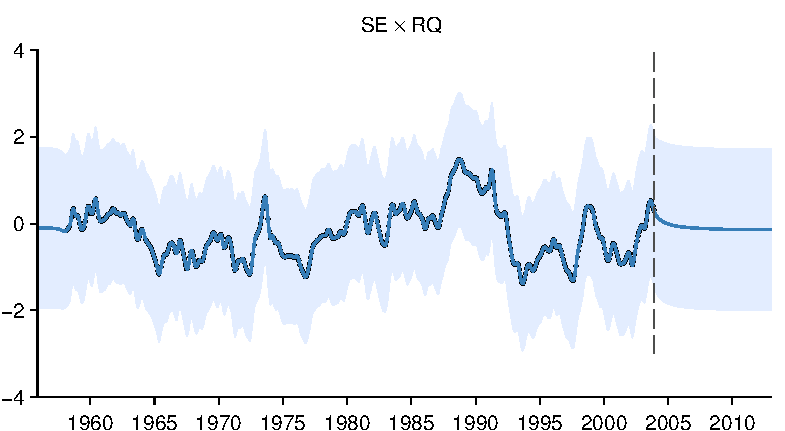
\includegraphics[trim=0cm 0cm 0cm 0cm, clip, width=0.35\columnwidth]{\descriptionfigsdir/old-gpss/03-mauna2003-s_3.pdf}}
    };
  \end{scope}  
  \begin{scope}[xshift=0.25\columnwidth]
  \draw[->,thick] (-0.04\columnwidth,0.05\columnwidth) -- (0.04\columnwidth,0.11\columnwidth); 
  \draw[->,thick] (-0.04\columnwidth,-0.05\columnwidth) -- (0.04\columnwidth,-0.11\columnwidth); 
  \end{scope}
  \begin{scope}[xshift=0.5\columnwidth]
    \begin{scope}[yshift=+0.15\columnwidth]
    \node [mybox] (box){
      \fbox{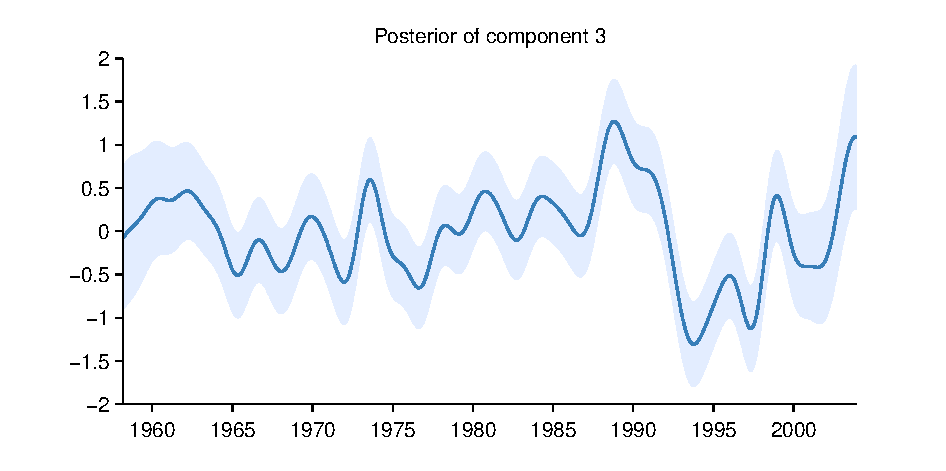
\includegraphics[trim=0cm 0cm 0cm 0cm, clip, width=0.35\columnwidth]{\descriptionfigsdir/03-mauna/03-mauna_3}}
    };
    \end{scope}
    \node[font=\LARGE] at (0,0) {$+$};
    \begin{scope}[yshift=-0.15\columnwidth]
    \node [mybox] (box){
      \fbox{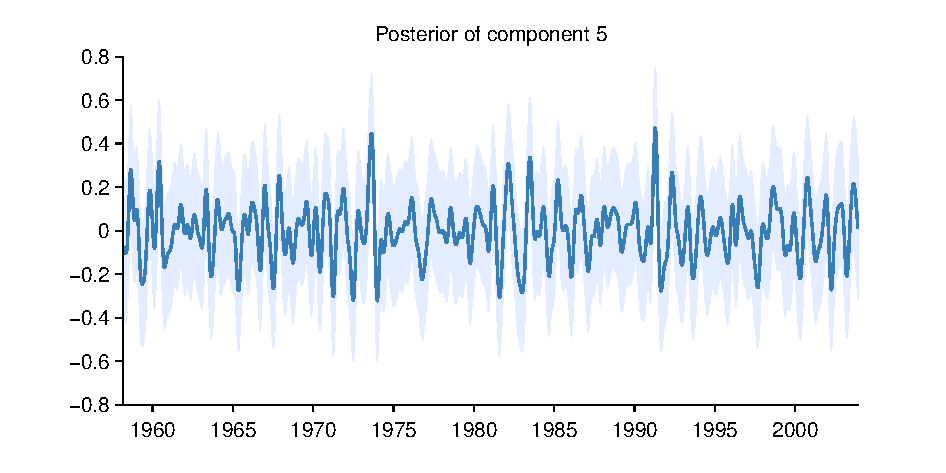
\includegraphics[trim=0cm 0cm 0cm 0cm, clip, width=0.35\columnwidth]{\descriptionfigsdir/03-mauna/03-mauna_5}}
    };
    \end{scope}
  \end{scope}
\end{tikzpicture}
\caption[Demonstration of rational quadratic kernel capturing multiple scales of variation on Mauna Loa data.]{
Left: Posterior of rational quadratic component of model for Mauna Loa data from chapter~\ref{ch:construction}.
Right: Posterior of two components found by \procedurename{} - the different scales of variation have been separated.
}
\label{fig:rq}
\end{figure}

An even more extreme pathological behaviour can be seen in figure~\ref{fig:description:rq_per} where a kernel of the form $\kRQ \kerntimes \kPer$ has explained a data set which \procedurename{} would more naturally described as a sum of a periodic component and uncorrelated noise.
The rational quadratic has introduced multiple lengthscales into the function allowing it to make a reasonable extrapolation of the periodicity in the data but also fit every data point perfectly.
For these reasons we exclude the rational quadratic kernel from our language.

\begin{figure}[ht]
  \centering
  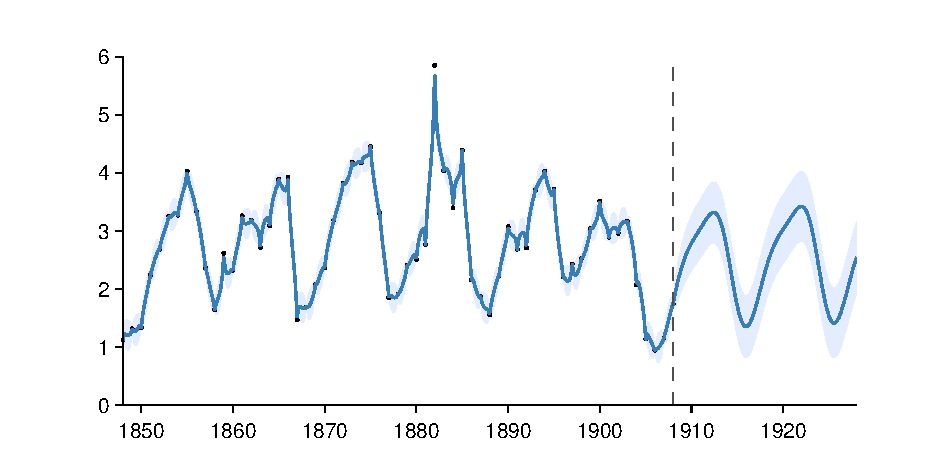
\includegraphics[trim=0cm 0cm 0cm 0cm, clip, width=0.8\columnwidth]{\descriptionfigsdir/old-gpss/mink_fur.pdf}
\caption[The pathological properties of the rational quadratic kernel when applied to mink fur sales data]{
Fit of a kernel of the form $\kRQ \kerntimes \kPer$ to mink fur sales data.
While this kernel produces good extrapolations of the average periodicity, it simulataneously `joins the dots', fitting all data points almost exactly.
It would be difficult to parsimoniously describe the properties of this function in words.
}
\label{fig:description:rq_per}
\end{figure}

At this point one may reasonably ask what the definition of `more natural' is.
I am using these phrases in the sense of attempting to produce a language of statistical models that match my own subjective biases.
By finding these pathological examples we are finding consequences of the grammar of kernels that do not match our subjective beliefs about the types of functions we expect to see.
While subjectivity is often less desirable than some form of objectivity when beginning a scientific investigation, it is probably better than biasing an analysis towards mathematically convenient forms that go against our subjective biases unless they can be proven to have good properties.
We discuss these philosophical points at greater length in section~\ref{sec:description:discussion}.

\paragraph{Subtraction of unnecessary constants}

The typical definition of the periodic ($\kPer$) kernel \citep[e.g.][]{Rasmussen2006-ml} used by \citet{Duvenaud2013-dn}, \citet{Kronberger_undated-vf} and in chapter~\ref{ch:construction}\footnote{and almost every other application of Gaussian processes to periodic data} is always greater than zero.
This is not necessary for the kernel to be positive semidefinite; we can subtract a constant from this kernel.
Similarly, the linear kernel used by \citet{Duvenaud2013-dn} and in chapter~\ref{ch:construction} contains a constant term that can be subtracted.

Without these constants subtracted we observe two main problems.
First, descriptions of products of kernels would become convoluted \eg $(\kPer + \kC) \times (\kLin + \kC) = \kC + \kPer + \kLin + \kPer \times \kLin$ is a sum of four qualitatively different functions (see section~\ref{sec:description:description} for justification that each of these kernels encodes for a distinct type of function).
Second, the constant functions can result in anti-correlation between components in the posterior, resulting in unnecessarily inflated credible intervals for each component which is shown in figure~\ref{fig:constant}.

\begin{figure}[ht]
\centering
\begin{tikzpicture}[]
  \begin{scope}[xshift=0.0\textwidth]
    \begin{scope}[yshift=+0.15\columnwidth]
    \node [mybox] (box){
      \fbox{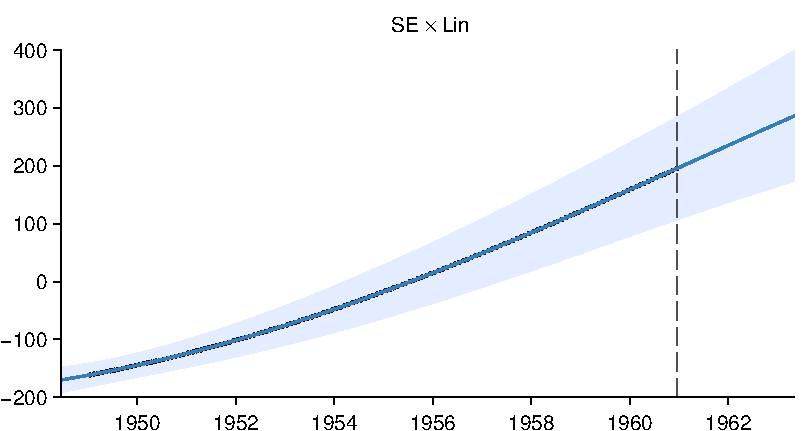
\includegraphics[trim=0cm 0cm 0cm 0cm, clip, width=0.35\columnwidth]{\descriptionfigsdir/old-gpss/01-airline-months_1.pdf}}
    };
    \end{scope}
    \node[font=\LARGE] at (0,0) {$+$};
    \begin{scope}[yshift=-0.15\columnwidth]
    \node [mybox] (box){
      \fbox{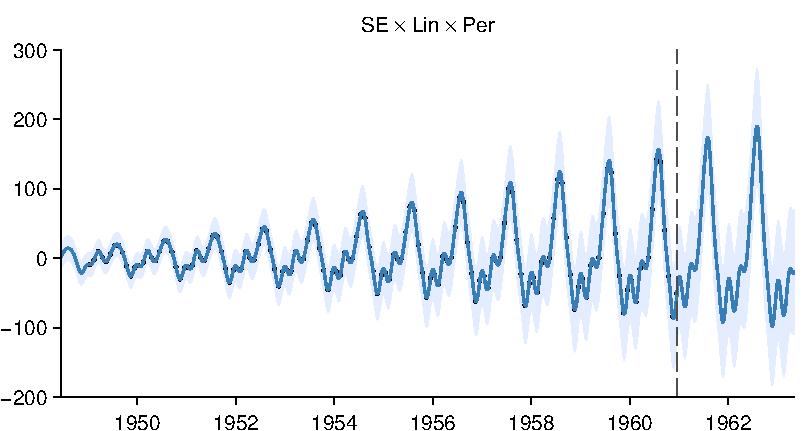
\includegraphics[trim=0cm 0cm 0cm 0cm, clip, width=0.35\columnwidth]{\descriptionfigsdir/old-gpss/01-airline-months_2.pdf}}
    };
    \end{scope}
  \end{scope}  
  \begin{scope}[xshift=0.25\columnwidth]
  \draw[->,thick] (-0.04\columnwidth,0.15\columnwidth) -- (0.04\columnwidth,0.15\columnwidth); 
  \draw[->,thick] (-0.04\columnwidth,-0.15\columnwidth) -- (0.04\columnwidth,-0.15\columnwidth); 
  \end{scope}
  \begin{scope}[xshift=0.5\columnwidth]
    \begin{scope}[yshift=+0.15\columnwidth]
    \node [mybox] (box){
      \fbox{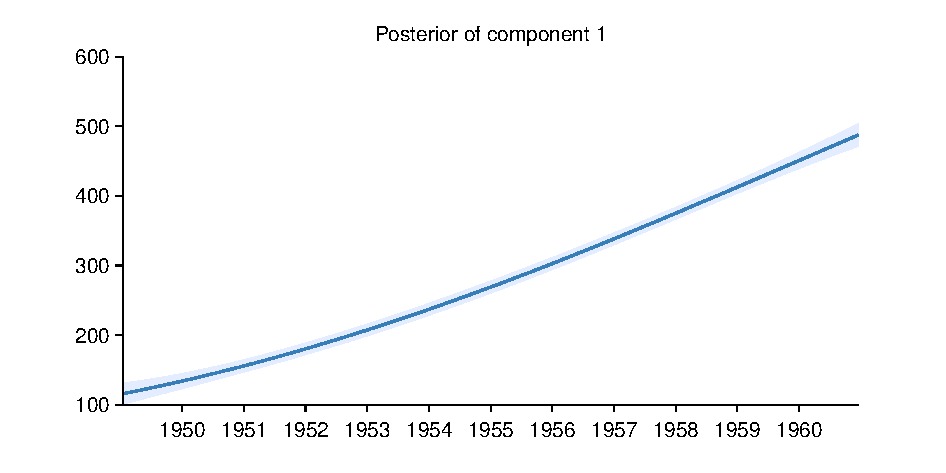
\includegraphics[trim=0cm 0cm 0cm 0cm, clip, width=0.35\columnwidth]{\descriptionfigsdir/01-airline/01-airline_1}}
    };
    \end{scope}
    \node[font=\LARGE] at (0,0) {$+$};
    \begin{scope}[yshift=-0.15\columnwidth]
    \node [mybox] (box){
      \fbox{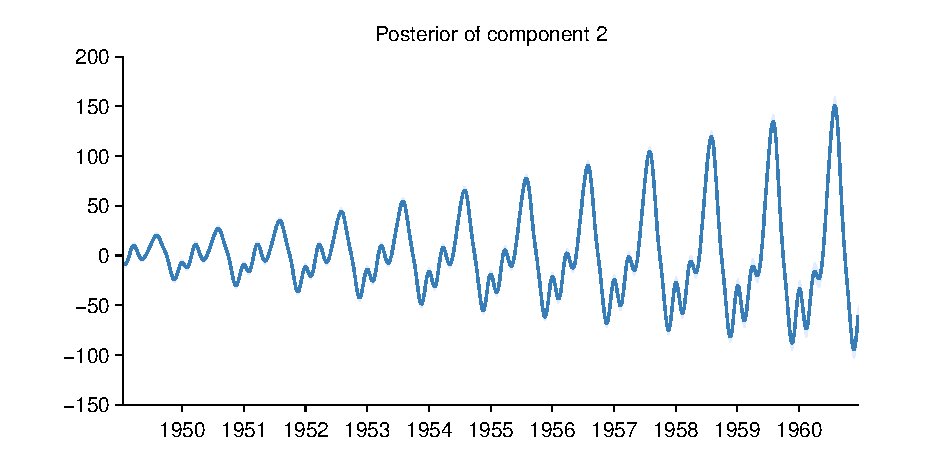
\includegraphics[trim=0cm 0cm 0cm 0cm, clip, width=0.35\columnwidth]{\descriptionfigsdir/01-airline/01-airline_2}}
    };
    \end{scope}
  \end{scope}
\end{tikzpicture}
\caption[Demonstration of inflated credible intervals when constants not removed from some kernels.]{
Left: Posterior of first two components for the airline passenger data from \citet{Duvenaud2013-dn} and chapter~\ref{ch:construction}.
Right: Posterior of first two components found by \procedurename{} - removing the constants from $\kLin$ and $\kPer$ has removed the inflated credible intervals due to anti-correlation in the posterior.
}
\label{fig:constant}
\end{figure}

\subsection{Properties of the new periodic kernel}

The newly defined zero-mean periodic kernel is given by
\[
  \kZMPer(\inputVar, \inputVar') =&  \sigma^2\frac{\exp\left(\frac{\cos\frac{2 \pi (\inputVar - \inputVar')}{p}}{\ell^2}\right) - I_0\left(\frac{1}{\ell^2}\right)}{\exp\left(\frac{1}{\ell^2}\right) - I_0\left(\frac{1}{\ell^2}\right)}
\]
where $I_0$ is the modified Bessel function of the first kind of order zero.
It is simply a carefully chosen linear transformation of the more common periodic kernel defined in equation~\ref{eq:kPer}.
A simple application of l'H\^opital's rule shows that
\begin{equation}
\kZMPer(x, x') \to \sigma^2\cos\left(\frac{2 \pi (x - x')}{p}\right) \quad \textrm{as} \quad\ell \to \infty.
\end{equation}
This limiting form is written as the cosine kernel ($\cos$).
It was recently demonstrated \citep{Wilson2013-eq} that any stationary kernel can be arbitrarily well approximated by kernels with expressions of the form
\begin{equation}
\sum \kSE \times \cos
\end{equation}
by appealing to Bochner's theorem \citep{Bochner1959-yk}.
By using this new periodic kernel our language of kernels also attains this completeness property.
Note that the infinite lengthscale ($\ell$) limit of the more common definition of the periodic kernel is a constant.

This version of the periodic kernel is now implemented in the GPML toolbox\footnotemark{} and is available at \url{gaussianprocess.org/gpml/code/matlab/cov/covPeriodicNoDC.m}
\footnotetext{\url{http://www.gaussianprocess.org/gpml/code/matlab/doc/}}

\subsection{Addition of the changepoint and changewindow operators}

In addition to these changes to the base kernels we also introduce changepoints into the language of kernels since they are a common phenomenon in time series (\eg figure~\ref{fig:periodic}).
We construct changepoints by assuming that the function we are attempting to model transitions between two different functions with the transition controlled by a sigmoidal function $\sigma$:
\[
  f(x) = \sigma(x)f_1(x) + (1 - \sigma(x))f_2(x).
\]
If we assume that $f_1 \sim \gp{}(0, k_1)$ and $f_2 \sim \gp{}(0, k_2)$ independently then $f \sim \gp{}(0, k)$ where
\[
  k(x, x') = \sigma(x)\sigma(x')k_1(x, x') + (1-\sigma(x))(1-\sigma(x'))k_2(x,x').
\]
We therefore define the changepoint operator as
\begin{align}
\kCP(\kernel_1, \kernel_2) = \kernel_1 \times \boldsymbol\sigma + \kernel_2 \times \boldsymbol{\bar\sigma}
\label{eq:cp}
\end{align}
where $\boldsymbol\sigma = \sigma(x)\sigma(x')$ and $\boldsymbol{\bar\sigma} = (1-\sigma(x))(1-\sigma(x'))$.
Not written are parameters of the sigmoid $\sigma$ that control its location and steepness.

We define changewindows $\kCW(\cdot,\cdot)$ similarly by replacing $\sigma(x)$ with a product of two sigmoids to create a `hat' function.
Examples of draws from Gaussian processes with kernels constructed using the changepoint operator are shown in figure~\ref{fig:description:cp}.

\begin{figure}[h]
\centering
\fbox{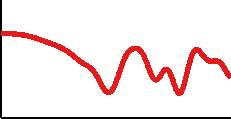
\includegraphics[width=0.22\columnwidth]{\descriptionfigsdir/cp/draw_1}}
\fbox{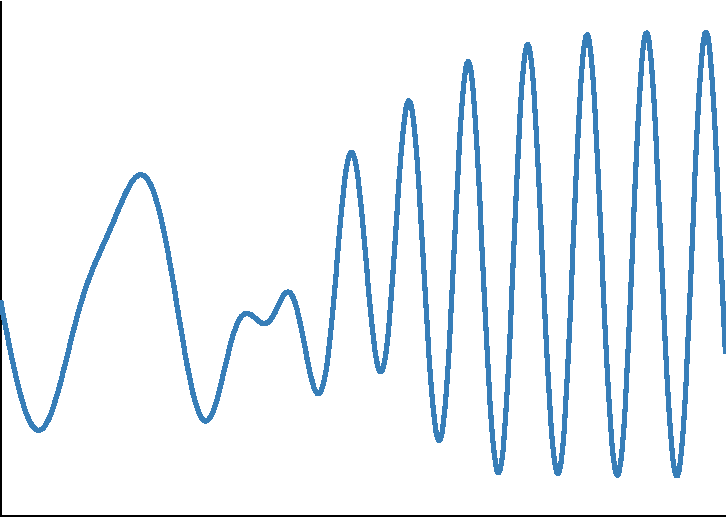
\includegraphics[width=0.22\columnwidth]{\descriptionfigsdir/cp/draw_2}}
\fbox{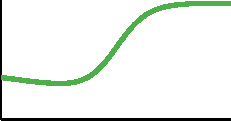
\includegraphics[width=0.22\columnwidth]{\descriptionfigsdir/cp/draw_3}}
\fbox{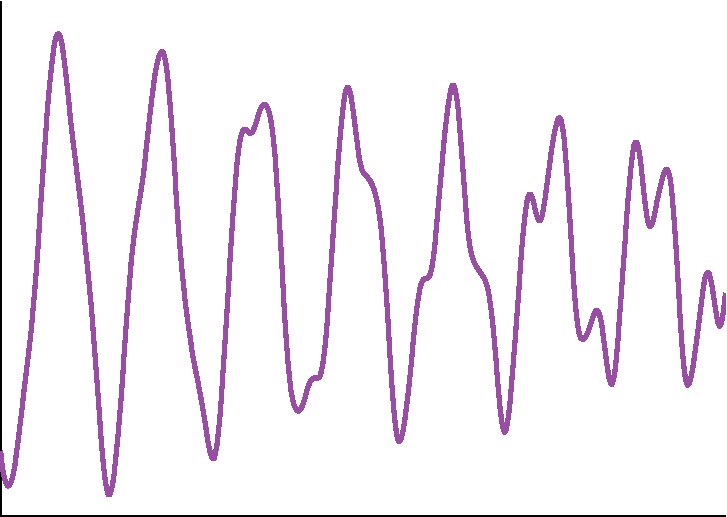
\includegraphics[width=0.22\columnwidth]{\descriptionfigsdir/cp/draw_4}}
\caption[Gaussian process samples with kernels formed using the changepoint operator.]{Examples of random samples from Gaussian processes with kernels constructed using the changepoint operator.}
\label{fig:description:cp}
\end{figure}

\subsection{Including heteroscedasticity}

In the language of kernels introduced in chapter~\ref{ch:construction} homoscedastic Gaussian noise was assumed for all models.
Gaussian noise is also a Gaussian process so we can introduce the noise model into the modelling language by introducing the white noise kernel
\[
\kWN(\inputVar, \inputVar') =& \sigma^2\delta_{\inputVar, \inputVar'}
\]
where $\delta_{\inputVar, \inputVar'}$ is the Kronecker delta function.
We use this as a base kernel and replace the model likelihood with a delta function.

Introducing the white noise kernel as a base kernel allows for the modelling language to express some forms of heteroscedasticity.
In particular, a $\kWN \kerntimes \kLin$ kernel encodes for uncorrelated Gaussian noise with linearly varying standard deviation.
The changepoint and changewindow operators also allow for heteroscedasticity when the noise model is included in the kernel.

\section{An updated language of  and search over regression models}
\label{sec:description:language}

%\gp{}s are distributions over functions such that any
%finite set of function evaluations, $(f(x_1), f(x_2), \ldots
%f(x_N))$, have a jointly Gaussian distribution
%\citep{rasmussen38gaussian}. A \gp{} is completely specified by its
%mean function, $\mu(x)=\mathbb{E}(f(x))$ and kernel (or covariance) function
%$\kernel(x,x') = \Cov(f(x),f(x'))$.
%It is common practice to assume zero mean,
%since marginalizing over an unknown mean function can be equivalently
%expressed as a zero-mean \gp{} with a new kernel. The structure of the
%kernel captures high-level properties of the unknown function, $f$,
%which in turn determines how the model generalizes or extrapolates to
%new data.  We can therefore define a language of regression models by
%specifying a language of kernels.

Since we have an updated set of base kernels and operators we review them.

\subsection{Base kernels}
\label{sec:description:base}

For scalar-valued inputs, the white noise ($\kWN$), constant ($\kC$), linear ($\kLin$), squared exponential ($\kSE$), and zero mean periodic kernels ($\kZMPer$) are defined as follows:
\begin{eqnarray}
\kWN(\inputVar, \inputVar') =& \sigma^2\delta_{\inputVar, \inputVar'} \\
\kC(\inputVar, \inputVar') =& \sigma^2 \\
\kLin(\inputVar, \inputVar') =& \sigma^2(\inputVar - \ell)(\inputVar' - \ell) \\
\kSE(\inputVar, \inputVar') =& \sigma^2\exp\left(-\frac{(\inputVar - \inputVar')^2}{2\ell^2}\right) \\
\kZMPer(\inputVar, \inputVar') =&  \sigma^2\frac{\exp\left(\frac{\cos\frac{2 \pi (\inputVar - \inputVar')}{p}}{\ell^2}\right) - I_0\left(\frac{1}{\ell^2}\right)}{\exp\left(\frac{1}{\ell^2}\right) - I_0\left(\frac{1}{\ell^2}\right)}
\end{eqnarray}
where $\delta_{\inputVar, \inputVar'}$ is the Kronecker delta function, $I_0$ is the modified Bessel function of the first kind of order zero and other symbols are parameters of the kernel functions.

\subsection{A larger language of regression models}

Table~\ref{table:motifs} lists common regression models that can be expressed by our language.
In this chapter we restrict to one dimensional functions (in particular, time series); the revised modelling language naturally extends into multiple dimensions in the manner described in chapter~\ref{ch:construction}.

\begin{table}[ht]
\centering
\begin{tabular}{l|l}
Regression model & Kernel \\
\midrule
\gp{} smoothing & $\kSE + \kWN$ \\
Linear regression & $\kC + \kLin + \kWN$ \\
Multiple kernel learning & $\sum \kSE$ + \kWN\\
Trend, cyclical, irregular & $\sum \kSE + \sum \kZMPer$ + \kWN\\
Fourier decomposition* & $\kC + \sum \cos$ + \kWN\\
Sparse spectrum \gp{}s* & $\sum \cos$ + \kWN\\
Spectral mixture* & $\sum \SE \times \cos$ + \kWN\\
Changepoints* & \eg $\kCP(\kSE, \kSE) + \kWN$ \\
Heteroscedasticity* & \eg $\kSE + \kLin \times \kWN$
\end{tabular}
\caption[Common regression models expressible in the \procedurename{} language.]{
Common regression models expressible in our language.
$\cos$ is a special case of $\kZMPer$.
* indicates a model that could not be expressed by the language defined in chapter~\ref{ch:construction}.
}
\label{table:motifs}
\end{table}

\subsection{Search operators}

The search operators introduced in chapter~\ref{ch:construction} are as follows:
%
\begin{eqnarray}
\mathcal{S} &\to& \mathcal{S} + \mathcal{B} \\
\mathcal{S} &\to& \mathcal{S} \times \mathcal{B} \\
\mathcal{B} &\to& \mathcal{B'}
\end{eqnarray}
%
where $\mathcal{S}$ represents any kernel subexpression and $\mathcal{B}$ is any base kernel \ie the search operators represent addition, multiplication and replacement.

To accommodate changepoint/window operators we introduce the following additional operators
%
\begin{eqnarray}
\mathcal{S} &\to& \kCP(\mathcal{S},\mathcal{S}) \\
\mathcal{S} &\to& \kCW(\mathcal{S},\mathcal{S}) \\
\mathcal{S} &\to& \kCW(\mathcal{S},\kC) \\
\mathcal{S} &\to& \kCW(\kC,\mathcal{S})
\end{eqnarray}
%
where $\kC$ is the constant kernel.
The last two operators result in a kernel only applying outside or within a certain region.

Based on experience with typical paths followed by the search algorithm we introduced the following operators
%
\begin{eqnarray}
\mathcal{S} &\to& \mathcal{S} \times (\mathcal{B} + \kC)\\
\mathcal{S} &\to& \mathcal{B}\\
\mathcal{S} + \mathcal{S'} &\to& \mathcal{S}\\
\mathcal{S} \times \mathcal{S'} &\to& \mathcal{S}
\end{eqnarray}
%
where $\mathcal{S'}$ represents any other kernel expression.
Their introduction is currently not rigorously justified.

\section{Automatic description of regression models}
\label{sec:description:description}

\paragraph{Overview}

In this section, we describe how \procedurename{} generates natural-language descriptions of the models found by the search procedure.
There are two main features of our language of \gp{} models that allow description to be performed automatically.

First, the sometimes complicated kernel expressions can be simplified into a sum of products.
A sum of kernels corresponds to a sum of functions so each product can be described separately.
Second, each kernel in a product modifies the resulting model in a consistent way.
Therefore, we can choose one kernel to be described as a noun, with all others described using adjectives or modifiers.

\paragraph{Sum of products normal form} 

We convert each kernel expression into a standard, simplified form.
We do this by first distributing all products of sums into a sum of products.
Next, we apply several simplifications to the kernel expression:
The product of two $\kSE$ kernels is another $\kSE$ with different parameters. Multiplying $\kWN$ by any stationary kernel ($\kC$, $\kWN$, $\kSE$, or $\kZMPer$) gives another $\kWN$ kernel. Multiplying any kernel by $\kC$ only changes the parameters of the original kernel.

After applying these rules, the kernel can as be written as a sum of terms of the form:
\begin{align*}
K \prod_m \kLin^{(m)} \prod_n \boldsymbol\sigma^{(n)},
\label{eq:sop}
\end{align*}
where $K$, if present, is one of \kWN, \kC, \kSE, $\prod_k \kZMPer^{(k)}$ or $\kSE \prod_k \kZMPer^{(k)}$
and $\prod_i\kernel^{(i)}$ denotes a product of kernels, each with different parameters.


\paragraph{Sums of kernels are sums of functions}
Formally, if $f_1(x) \dist \gp{}(0, \kernel_1)$ and independently $f_2(x) \dist \gp{}(0, \kernel_2)$ then ${f_1(x) + f_2(x) \dist \gp{}(0, \kernel_1 + \kernel_2)}$.
This lets us describe each product of kernels separately just as we plotted separate additive components in chapter~\ref{ch:construction}

\paragraph{Each kernel in a product modifies a model in a consistent way}
This allows us to describe the contribution of each kernel as a modifier of a noun phrase.
These descriptions are summarised in table~\ref{table:modifiers} and justified below:

\begin{itemize}
\item {\bf Multiplication by $\kSE$} removes long range correlations from a model since $\kSE(x,x')$ decreases monotonically to 0 as $|x - x'|$ increases.
This will convert any global correlation structure into local correlation only.
\item {\bf Multiplication by $\kLin$} is equivalent to multiplying the function being modelled by a linear function.
If $f(x) \dist \gp{}(0, \kernel)$, then $xf(x) \dist \gp{}\left(0, k \times \kLin \right)$.
This causes the standard deviation of the model to vary linearly without affecting the correlation.
\item {\bf Multiplication by $\boldsymbol\sigma$} is equivalent to multiplying the function being modelled by a sigmoid which means that the function goes to zero before or after some point.
\item {\bf Multiplication by $\kZMPer$}
modifies the correlation structure in the same way as multiplying the function by an independent periodic function.
Formally, if ${f_1(x) \dist \gp{}(0, \kernel_1)}$ and ${f_2(x) \dist \gp{}(0, \kernel_2)}$ then
\begin{align}
{\textrm{Cov} \left[f_1(x)f_2(x), f_1(x')f_2(x') \right] = k_1(x,x')k_2(x,x')}.\nonumber
\end{align}
We note however that since this multiplication affects only the correlation structure, the description given in table~\ref{table:modifiers} is somewhat loose.
\end{itemize}

\begin{table}[ht]
\centering
\begin{tabular}{l|l}
Kernel & Postmodifier phrase \\
\midrule
$\kSE$  & whose shape changes smoothly \\
$\kZMPer$ & modulated by a periodic function \\
$\kLin$ & with linearly varying amplitude \\
$\prod_k \kLin^{(k)}$ & with polynomially varying amplitude \\
$\prod_k \boldsymbol{\sigma}^{(k)}$ & which applies until / from [changepoint] \\
\end{tabular}
\caption[Postmodifier descriptions of each kernel.]{
Postmodifier descriptions of each kernel
}
\label{table:modifiers}
\end{table}

\paragraph{Constructing a complete description of a product of kernels}
We choose one kernel to act as a noun which is then described by the functions it encodes for when unmodified (see table~\ref{table:nouns}).
Modifiers corresponding to the other kernels in the product are then appended to this description, forming a noun phrase of the form:
\begin{align*}
\textnormal{Determiner}	+	\textnormal{Premodifiers} +	\textnormal{Noun}	+	\textnormal{Postmodifiers}
\end{align*}

As an example, a kernel of the form $\kZMPer \times  \kLin \times \boldsymbol{\sigma}$ could be described as a
\begin{align*}
\underbrace{\kZMPer}_{\textnormal{\scriptsize periodic function}} \times 
\underbrace{\kLin}_{\textnormal{\scriptsize with linearly varying amplitude}} \times 
\underbrace{\boldsymbol{\sigma}}_{\textnormal{\scriptsize which applies until 1700.}}
\end{align*}
where $\kZMPer$ has been selected as the head noun.

\begin{table}[ht]
\centering
\begin{tabular}{l|l}
Kernel & Noun phrase \\
\midrule
$\kWN$  & uncorrelated noise \\
$\kC$   & constant \\
$\kSE$  & smooth function \\
$\kZMPer$ & periodic function \\
$\kLin$ & linear function \\
$\prod_k \kLin^{(k)}$ & polynomial \\
\end{tabular}
\caption[Noun phrase descriptions of each kernel]{
Noun phrase descriptions of each kernel
}
\label{table:nouns}
\end{table}

\paragraph{Refinements to the descriptions}

There are a number of ways in which the descriptions of the kernels can be made more interpretable and informative:
\begin{itemize}
  \item Which kernel is chosen as the head noun can change the interpretability of a description.
  \item Descriptions can change qualitatively according to kernel parameters \eg `a rapidly varying smooth function'.
  \item Descriptions can include kernel parameters \eg `modulated by a periodic function with a period of [period]'.
  \item Descriptions can include extra information calculated from data \eg `a linearly increasing function'.
  \item Some kernels can be described as premodifiers \eg `an approximately periodic function'.
\end{itemize}

The reports in the supplementary material and in section~\ref{sec:examples} include some of these refinements.
For example, the head noun is chosen according to the following ordering:
\begin{align*}
\kZMPer > \kWN, \kSE, \kC > \prod_m \kLin^{(m)} > \prod_n \boldsymbol\sigma^{(n)}
\end{align*}
\ie $\kZMPer$ is always chosen as the head noun when present.
The parameters and design choices of these refinements have been chosen by our best judgement, but learning these parameters objectively from expert statisticians would be an interesting area for future study.

\paragraph{Ordering additive components}

The reports generated by \procedurename{} attempt to present the most interesting or important features of a data set first.
As a heuristic, we order components by always adding next the component which most reduces the 10-fold cross-validated mean absolute error.

\subsection{Worked example}

Suppose we start with a kernel of the form
\begin{align*}
\kSE \times (\kWN \times \kLin + \kCP(\kC, \kZMPer)).
\end{align*}
This is converted to a sum of products:
\begin{align*}
\kSE \times \kWN \times \kLin + \kSE \times \kC \times \boldsymbol{\sigma} + \kSE \times \kZMPer \times \boldsymbol{\bar\sigma}.
\end{align*}
which is simplified to
\begin{align*}
\kWN \times \kLin + \kSE \times \boldsymbol{\sigma} + \kSE \times \kZMPer \times \boldsymbol{\bar\sigma}.
\end{align*}

To describe the first component, the head noun description for $\kWN$, `uncorrelated noise', is concatenated with a modifier for $\kLin$, `with linearly increasing amplitude'.
The second component is described as `A smooth function with a lengthscale of [lengthscale] [units]', corresponding to the $\kSE$, `which applies until [changepoint]', which corresponds to the $\boldsymbol{\sigma}$.
Finally, the third component is described as `An approximately periodic function with a period of [period] [units] which applies from [changepoint]'.


\section{Example descriptions of time series}
\label{sec:examples}
We demonstrate the ability of our procedure to discover and describe a variety of patterns on two time series.
An example of a full automatically-generated report is provided in appendix~\ref{ch:example-solar}.

\subsection{Summarizing 400 Years of Solar Activity}
\label{sec:solar}

\begin{figure}[h]
\centering
\includegraphics[trim=0.2cm 18.0cm 8cm 2cm, clip, width=0.8\columnwidth]{\descriptionfigsdir/solarpages/pg_0002-crop}
\caption[Solar irradiance data]{
Solar irradiance data.}
\label{fig:solar}
\end{figure}

We show excerpts from the report automatically generated on annual solar irradiation data from 1610 to 2011 (figure~\ref{fig:solar}).
This time series has two pertinent features: a roughly 11-year cycle of solar activity, and a period lasting from 1645 to 1715 with much smaller variance than the rest of the dataset.
This flat region is known as the Maunder minimum, a period in which sunspots were extremely rare \citep{Lean1995-vp}.
\procedurename{} clearly identifies these two features, as discussed below.

\begin{figure}[h]
\centering
\fbox{\includegraphics[trim=0cm 10.8cm 0cm 6.3cm, clip, width=0.98\columnwidth]{\descriptionfigsdir/solarpages/pg_0002-crop}}
\caption[Summaries generated by \procedurename{} for the solar irradiance data.]{
Automatically generated descriptions of the components discovered by \procedurename{} on the solar irradiance data set.
The dataset has been decomposed into diverse structures with simple descriptions.}
\label{fig:exec}
\end{figure}
Figure \ref{fig:exec} shows the natural-language summaries of the top four components chosen by \procedurename{}.
From these short summaries, we can see that our system has identified the Maunder minimum (second component) and 11-year solar cycle (fourth component).
These components are visualised in figures~\ref{fig:maunder} and \ref{fig:periodic}, respectively. 
The third component corresponds to long-term trends, as visualised in figure~\ref{fig:smooth}.

\begin{figure}[ht]
\centering
\fbox{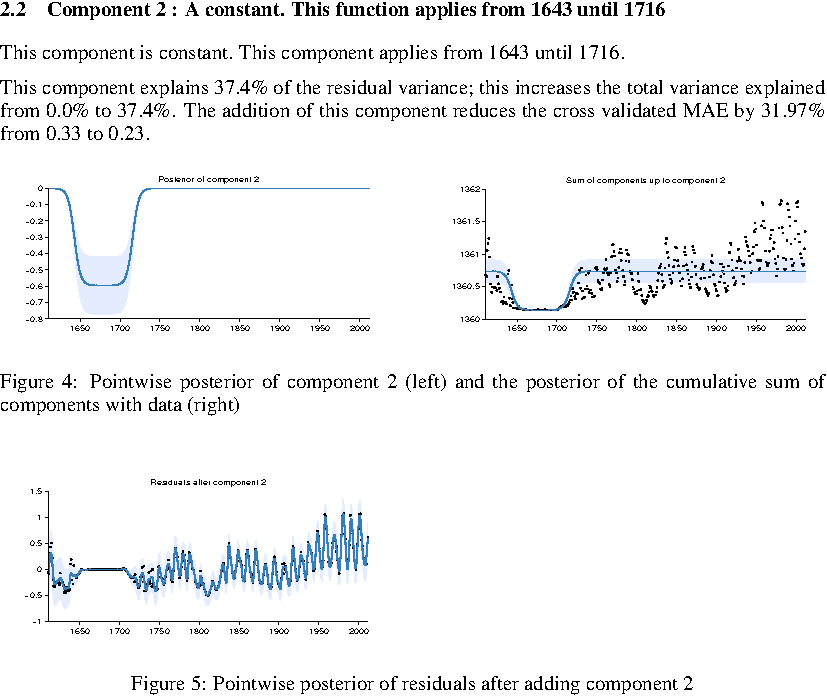
\includegraphics[trim=0cm 4.75cm 0cm 0.7cm, clip, width=0.98\columnwidth]{\descriptionfigsdir/solarpages/pg_0005-crop}}
\caption[Automatic identification of the Maunder minimum.]{One of the learned components corresponds to the Maunder minimum.}
\label{fig:maunder}
\end{figure}

\begin{figure}[h!]
\centering
\fbox{\includegraphics[trim=0cm 4.75cm 0cm 1cm, clip, width=0.98\columnwidth]{\descriptionfigsdir/solarpages/pg_0006-crop}}
\caption[Characterising the medium-term smoothness of solar activity levels.]{Characterising the medium-term smoothness of solar activity levels.  By allowing other components to explain the periodicity, noise, and the Maunder minimum, \procedurename{} can isolate the part of the signal best explained by a slowly-varying trend.}
\label{fig:smooth}
\end{figure}

\begin{figure}[ht]
\centering
\fbox{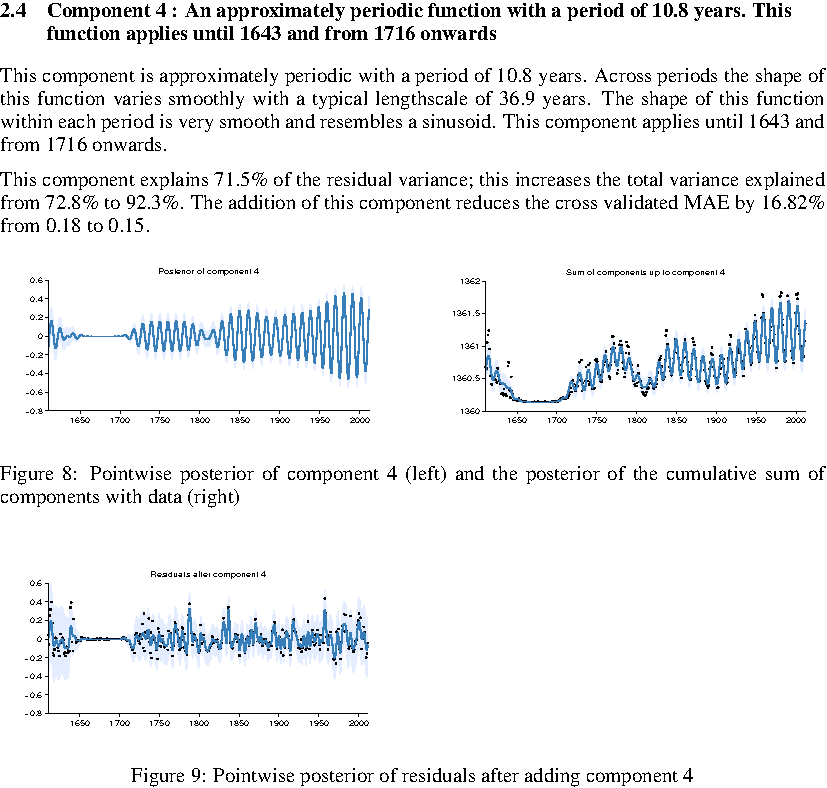
\includegraphics[trim=0cm 4.75cm 0cm 1.0cm, clip, width=0.98\columnwidth]{\descriptionfigsdir/solarpages/pg_0007-crop}}
\caption[Automatic identification of solar cycles.]{
Extract from an automatically-generated report describing the model components discovered by \procedurename{}.
This part of the report isolates and describes the approximately 11-year sunspot cycle, also noting its disappearance during the 16th century, a time known as the Maunder minimum \citep{Lean1995-vp}.
}
\label{fig:periodic}
\end{figure}

\subsection{Finding heteroscedasticity in air traffic data}
\label{sec:airline}

\begin{figure}[h]
\centering
\includegraphics[trim=0.4cm 16.8cm 8cm 2cm, clip, width=0.8\columnwidth]{\descriptionfigsdir/airlinepages/pg_0002-crop}
\caption[Airline data.]{
International airline passenger monthly volume \citep[e.g.][]{Box1976-qk}.}
\label{fig:airline}
\end{figure}

Next, we present the analysis generated by our procedure on international airline passenger data (figure~\ref{fig:airline}).
The model constructed by \procedurename{} has four components: $\kLin + \kSE \times \kZMPer \times \kLin + \kSE + \kWN \times \kLin$, with descriptions given in figure~\ref{fig:exec-airline}.

\begin{figure}[h]
\centering
\fbox{\includegraphics[trim=0cm 6.8cm 0cm 6cm, clip, width=0.98\columnwidth]{\descriptionfigsdir/airlinepages/pg_0002-crop}}
\caption[Summaries produced by \procedurename{} for the airline data.]{
Short descriptions and summary statistics for the four components of the airline model.}
\label{fig:exec-airline}
\end{figure}

The second component (figure~\ref{fig:lin_periodic}) is accurately described as approximately ($\kSE$) periodic ($\kZMPer$) with linearly increasing amplitude ($\kLin$).
%
\begin{figure}[h]
\centering
\fbox{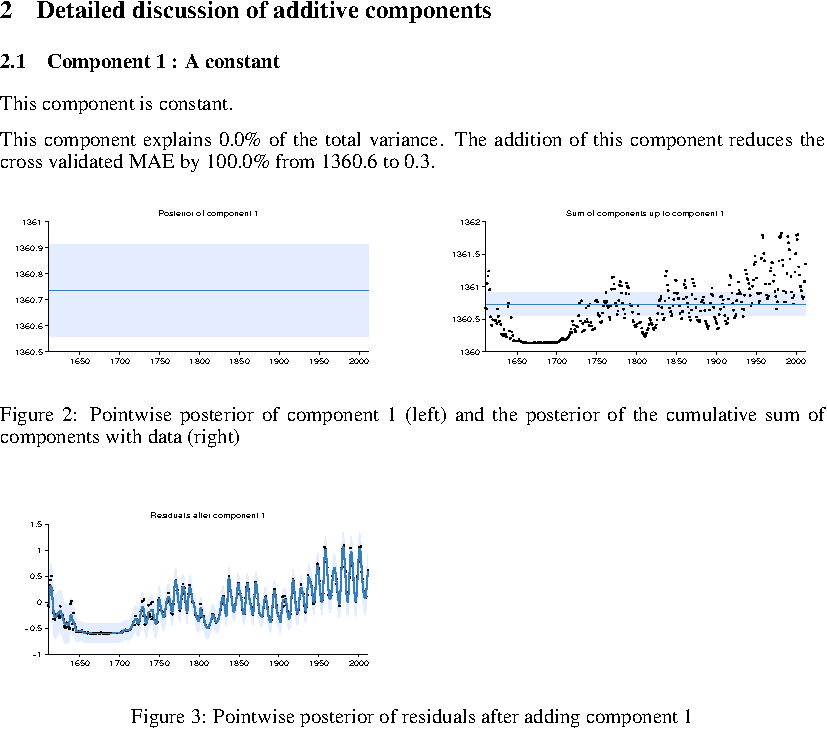
\includegraphics[trim=0cm 4.75cm 0cm 0cm, clip, width=0.98\columnwidth]{\descriptionfigsdir/airlinepages/pg_0004-crop}}
\caption{Capturing non-stationary periodicity in the airline data.}
\label{fig:lin_periodic}
\end{figure}
%
By multiplying a white noise kernel by a linear kernel, the model is able to express heteroscedasticity (figure~\ref{fig:heteroscedastic}).
%
\begin{figure}[h]
\centering
\fbox{\includegraphics[trim=0cm 0cm 0cm 0cm, clip, width=0.98\columnwidth]{\descriptionfigsdir/airlinepages/pg_0006-crop}}
\caption{Modeling heteroscedasticity in the airline data.}
\label{fig:heteroscedastic}
\end{figure}

\subsection{Comparison to equation learning}
\label{sec:eqn-learning-comp}

We now compare the descriptions generated by \procedurename{} to parametric functions produced by an equation learning system.
We show equations produced by Eureqa \citep{Nutonian2011-el} for the data sets shown above, using the default mean absolute error performance metric.

The learned function for the solar irradiance data is
\begin{align*}
\textrm{Irradiance($t$)} = 1361 + \alpha\sin(\beta + \gamma t)\sin(\delta + \epsilon t^2 - \zeta t)
\end{align*}
where $t$ is time and constants are replaced with symbols for brevity.
This equation captures the constant offset of the data, and models the long-term trend with a product of sinusoids, but fails to capture the solar cycle or the Maunder minimum.%\fTBD{Plot if you can find the data}.

The learned function for the airline passenger data is
\begin{align*}
\textrm{Passengers($t$)} = \alpha t + \beta\cos(\gamma - \delta t)\textrm{logistic}(\epsilon t - \zeta) - \eta
\end{align*}
which captures the approximately linear trend, and the periodic component with approximately linearly (logistic) increasing amplitude.
However, the annual cycle is heavily approximated by a sinusoid and the model does not capture heteroscedasticity.

\section{Related work}
\label{sec:related-work}

Section~\ref{sec:construction:related_work} describes work most closely related to the construction of Gaussian process models with complex kernels.
In this section we review work relating to systems producing natural language output and the automation of data analysis.

\paragraph{Natural-language output}
To the best of our knowledge, our procedure is the first example of automatic description of nonparametric statistical models.
However, systems with natural language output have been built in the areas of scene interpretation \citep{Karpathy_undated-ww}, video interpretation \citep{Barbu2012-wv} and automated theorem proving \citep{Ganesalingam_undated-us}.

\paragraph{Automatic machine learning}

Our work joins a growing literature attempting to automate various aspects of machine learning.
\citet{Thornton2013-zg} present AutoWEKA, a system which automates model selection in the data analysis software WEKA.
Similarly the Google prediction API \citep{green2011prediction} provides an API which hides the model selection and optimisation aspects of making predictions given training data.
In a more restricted but no less important context, \citet{Snoek2012-ri} demonstrated how Bayesian optimisation techniques could be used to tune the parameters of machine learning methods automatically, improving upon state of the art performance in a number of domains merely by improved parameter tuning.
Our work moves this line of research forward by attempting to automatically explain a data set as well as building a model with good predictive performance.

\section{Predictive Accuracy}
\label{sec:numerical}

\begin{figure*}[ht]
\centering
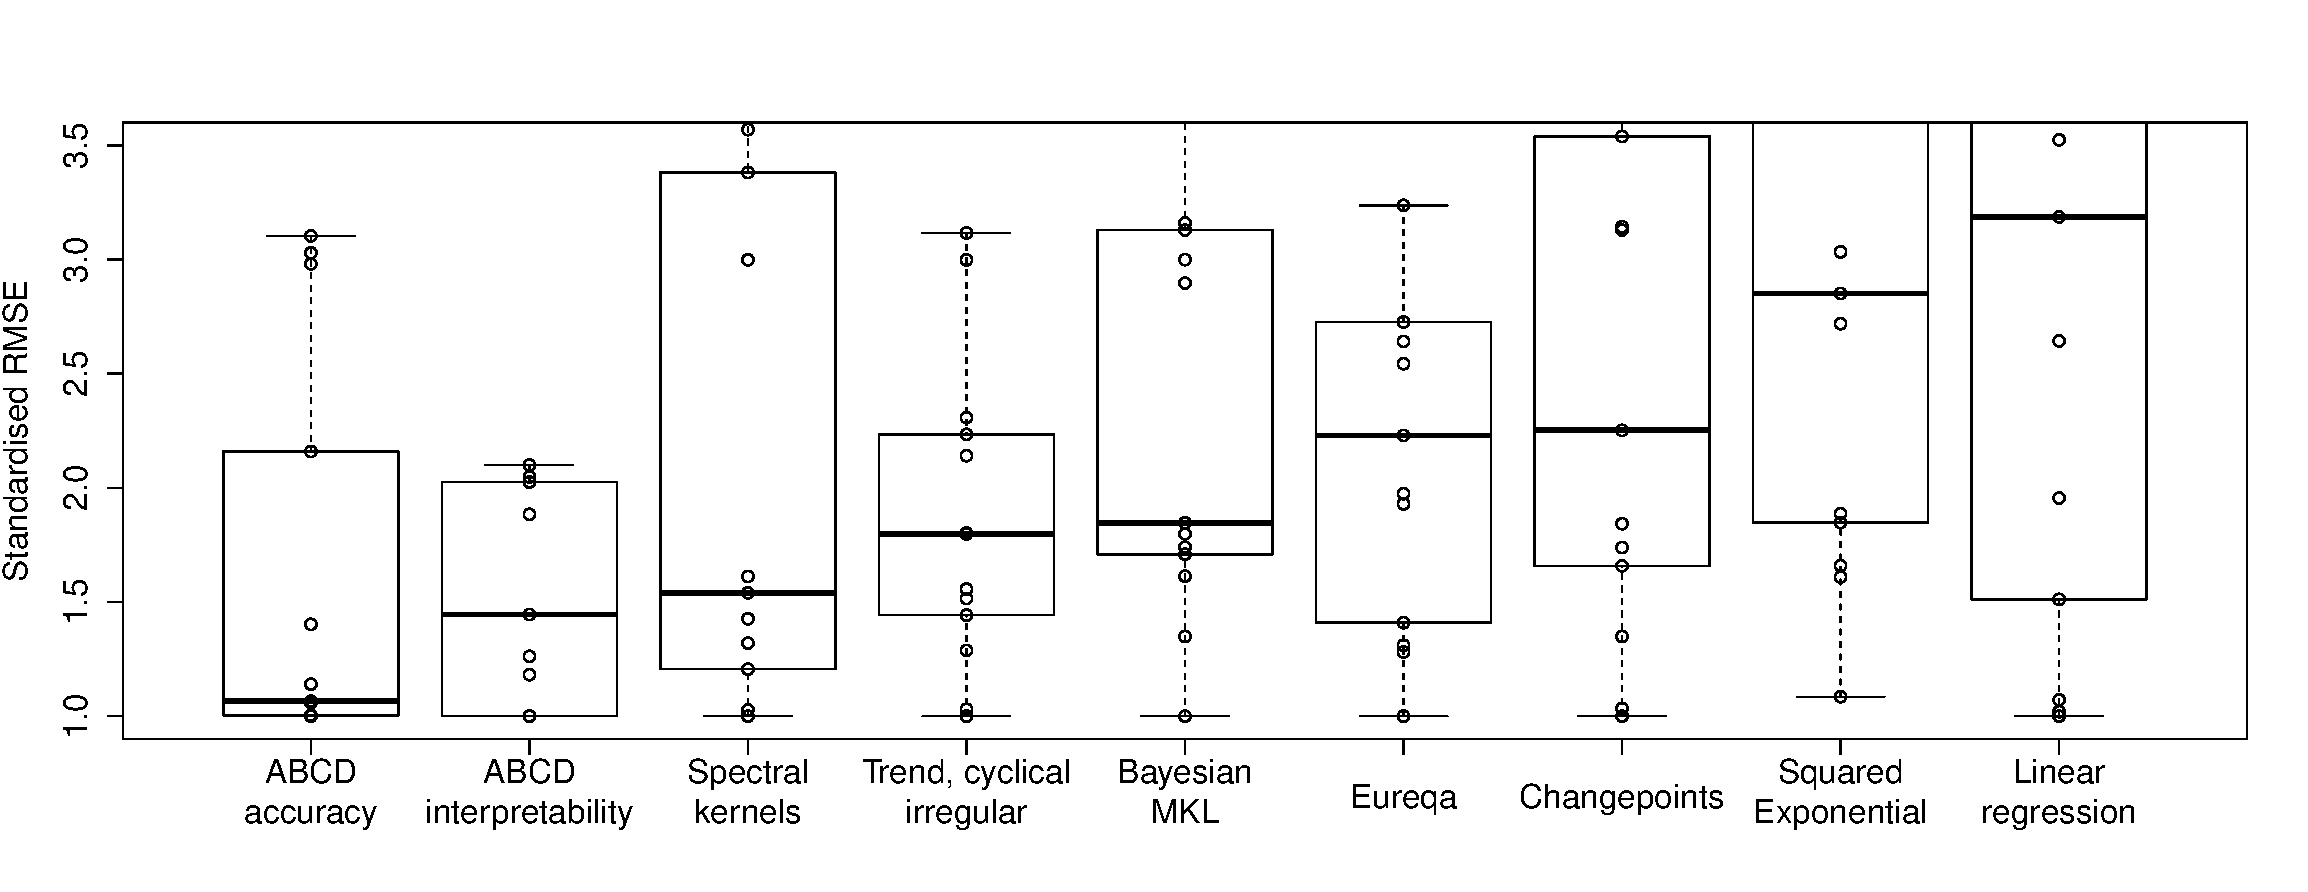
\includegraphics[width=\textwidth]{\descriptionfigsdir/box_extrap_wide}
\vspace{-0.8cm}
\caption[RMSE comparison of \procedurename{} and other algorithms at extrapolation.]{
Raw data, and box plot (showing median and quartiles) of standardised extrapolation RMSE (best performance = 1) on 13 time-series.
The methods are ordered by median.
}
\label{fig:box_extrap_dist}
\end{figure*}

In addition to our demonstration of the interpretability of \procedurename{}, we compared the predictive accuracy of various model-building algorithms at interpolating and extrapolating time-series.
\procedurename{} outperforms the other methods on average.

\paragraph{Data sets}

We evaluate the performance of the algorithms listed below on 13 real time-series from various domains from the time series data library \citep{Hyndman_undated-zj}; plots of the data can be found in appendix~\ref{ch:datasets}.

\paragraph{Algorithms}

We compare \procedurename{} to equation learning using Eureqa \citep{Nutonian2011-el} and six other regression algorithms: linear regression, \gp{} regression with a single $\kSE$ kernel (squared exponential), a Bayesian variant of multiple kernel learning (MKL) \citep[e.g.][]{Bach2004-lb}, change point modeling \citep[e.g.][]{Garnett2010-rd, Saatci2010-el, Fox2012-fm}, spectral mixture kernels \citep{Wilson2013-eq} (spectral kernels) and trend-cyclical-irregular models \citep[e.g.][]{Lind2006-th}.

The spans of the languages of kernels of the language used by \procedurename{} and the kernel search introduced in chapter~\ref{ch:description} are very similar; the changes are close to being only a change of basis.
Consequently their predictive accuracy is nearly identical so we only include \procedurename{} in the results for brevity.

We use the default mean absolute error criterion when using Eureqa.
All other algorithms can be expressed as restrictions of our modelling language (see table~\ref{table:motifs}) so we perform inference using the same search methodology and selection criterion\footnotemark~with appropriate restrictions to the language.
For MKL, trend-cyclical-irregular and spectral kernels, the greedy search procedure of \procedurename{} corresponds to a forward-selection algorithm.
For squared exponential and linear regression the procedure corresponds to marginal likelihood optimisation.
More advanced inference methods are typically used for changepoint modelling but we use the same inference method for all algorithms for comparability.
\footnotetext{We experimented with using unpenalised marginal likelihood as the search criterion but observed overfitting, as is to be expected.} 

We restricted to regression algorithms for comparability; this excludes models which regress on previous values of times series, such as autoregressive or moving-average models \citep[e.g.][]{Box1976-qk}.
Constructing a language for this class of time-series model would be an interesting area for future research.

\paragraph{Interpretability versus accuracy}

BIC trades off model fit and complexity by penalising the number of parameters in a kernel expression.
This can result in \procedurename{} favouring kernel expressions with nested products of sums, producing descriptions involving many additive components.
While these models have good predictive performance the large number of components can make them less easy to interpret.
We experimented with distributing all products over addition during the search, causing models with many additive components to be more heavily penalised by BIC.
We call this procedure \procedurename{}-interpretability, in contrast to the unrestricted version of the search, \procedurename{}-accuracy.

\paragraph{Extrapolation}

To test extrapolation we trained all algorithms on the first 90\% of the data, predicted the remaining 10\% and then computed the root mean squared error (RMSE).
The RMSEs are then standardised by dividing by the smallest RMSE for each data set so that the best performance on each data set will have a value of 1.

Figure~\ref{fig:box_extrap_dist} shows the standardised RMSEs across algorithms.
\procedurename{}-accuracy outperforms \procedurename{}-interpretability but both versions have lower quartiles than all other methods.

Overall, the model construction methods with greater capacity perform better: \procedurename{} outperforms trend-cyclical-irregular, which outperforms Bayesian MKL, which outperforms squared exponential.
Despite searching over a rich model class, Eureqa performs relatively poorly, since very few datasets are parsimoniously explained by a parametric equation.

Not shown on the plot are large outliers for spectral kernels, Eureqa, squared exponential and linear regression with values of 11, 493, 22 and 29 respectively.
All of these outliers occurred on a data set with a large discontinuity (see the call centre data in appendix~\ref{ch:datasets}).

\paragraph{Interpolation}

To test the ability of the methods to interpolate, we randomly divided each data set into equal amounts of training data and testing data.
We trained each algorithm on the training half of the data, produced predictions for the remaining half and then computed the root mean squared error (RMSE).
The values of the RMSEs are then standardised by dividing by the smallest RMSE for each data set \ie the best performance on each data set will have a value of 1.

Figure~\ref{fig:box_interp} shows the standardised RMSEs for the different algorithms.
The box plots show that all quartiles of the distribution of standardised RMSEs are lower for both versions of \procedurename{}.
The median for \procedurename{}-accuracy is 1; it is the best performing algorithm on 7 datasets.
The largest outliers of \procedurename{} and spectral kernels are similar in value.

\begin{figure*}[ht]
\centering
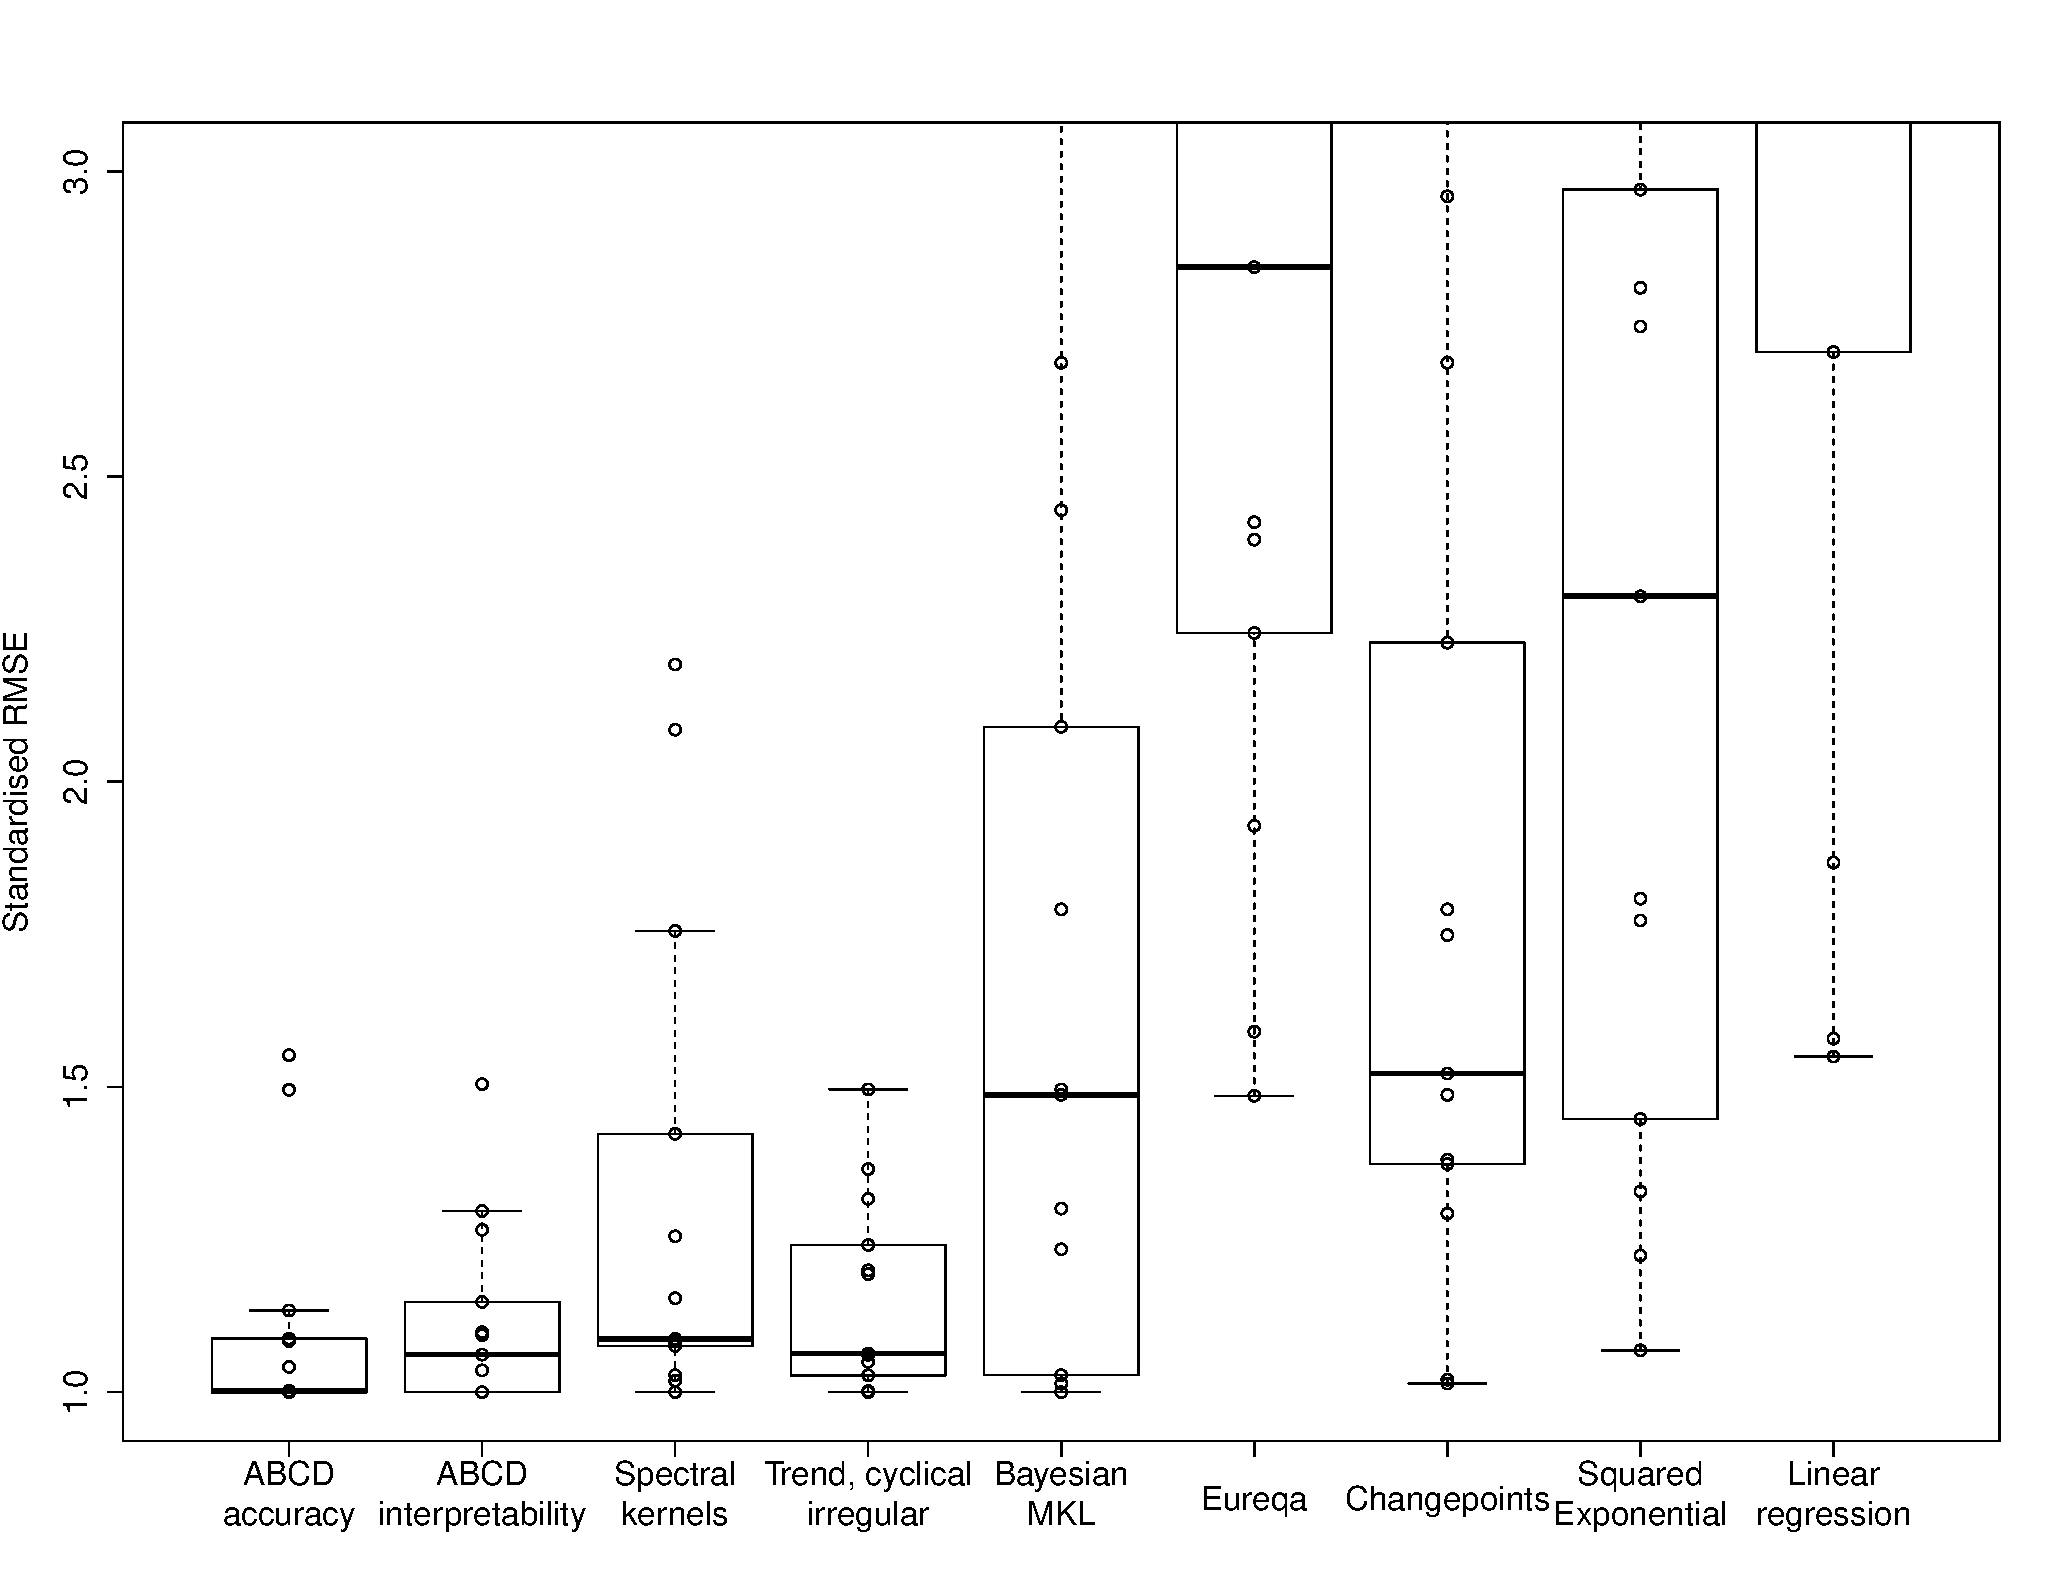
\includegraphics[width=\textwidth]{\descriptionfigsdir/box_interp}
\caption[RMSE comparison of \procedurename{} and other algorithms at interpolation.]{
Box plot of standardised RMSE (best performance = 1) on 13 interpolation tasks.
}
\label{fig:box_interp}
\end{figure*}

Changepoints performs slightly worse than MKL despite being strictly more general than Changepoints.
The introduction of changepoints allows for more structured models, but it introduces parametric forms into the regression models (\ie the sigmoids expressing the changepoints).
This results in worse interpolations at the locations of the change points, suggesting that a more robust modelling language would require a more flexible class of changepoint shapes or improved inference (\eg fully Bayesian inference over the location and shape of the changepoint).

Eureqa is not suited to this task and performs poorly.
The models learned by Eureqa tend to capture only broad trends of the data since the fine details are not well explained by parametric forms.

\subsection{Tables of standardised RMSEs}

See table~\ref{table:interp} for raw interpolation results and table~\ref{table:extrap} for raw extrapolation results. 
The rows follow the order of the datasets in appendix~\ref{ch:datasets}.
The following abbreviations are used: \procedurename{}-accuracy (\procedurename{}-acc), \procedurename{}-interpretability ((\procedurename{}-int), Spectral kernels (SP), Trend-cyclical-irregular (TCI), Bayesian MKL (MKL), Eureqa (EL), Changepoints (CP), Squared exponential (SE) and Linear regression (Lin).

\begin{table}[ht]
\center
\begin{tabular}{|c|c|c|c|c|c|c|c|c|}
\hline
\procedurename{}-acc & \procedurename{}-int & SP & TCI & MKL & EL & CP & SE & Lin \\
\hline
1.04 & 1.00 & 2.09 & 1.32 & 3.20 & 5.30 & 3.25 & 4.87 & 5.01\\
1.00 & 1.27 & 1.09 & 1.50 & 1.50 & 3.22 & 1.75 & 2.75 & 3.26\\
1.00 & 1.00 & 1.09 & 1.00 & 2.69 & 26.20 & 2.69 & 7.93 & 10.74\\
1.09 & 1.04 & 1.00 & 1.00 & 1.00 & 1.59 & 1.37 & 1.33 & 1.55\\
1.00 & 1.06 & 1.08 & 1.06 & 1.01 & 1.49 & 1.01 & 1.07 & 1.58\\
1.50 & 1.00 & 2.19 & 1.37 & 2.09 & 7.88 & 2.23 & 6.19 & 7.36\\
1.55 & 1.50 & 1.02 & 1.00 & 1.00 & 2.40 & 1.52 & 1.22 & 6.28\\
1.00 & 1.30 & 1.26 & 1.24 & 1.49 & 2.43 & 1.49 & 2.30 & 3.20\\
1.00 & 1.09 & 1.08 & 1.06 & 1.30 & 2.84 & 1.29 & 2.81 & 3.79\\
1.08 & 1.00 & 1.15 & 1.19 & 1.23 & 42.56 & 1.38 & 1.45 & 2.70\\
1.13 & 1.00 & 1.42 & 1.05 & 2.44 & 3.29 & 2.96 & 2.97 & 3.40\\
1.00 & 1.15 & 1.76 & 1.20 & 1.79 & 1.93 & 1.79 & 1.81 & 1.87\\
1.00 & 1.10 & 1.03 & 1.03 & 1.03 & 2.24 & 1.02 & 1.77 & 9.97\\
\hline
\end{tabular}
\caption{Interpolation standardised RMSEs.}
\label{table:interp}
\end{table}

\begin{table}[ht]
\center
\begin{tabular}{|c|c|c|c|c|c|c|c|c|}
\hline
\procedurename{}-acc & \procedurename{}-int & SP & TCI & MKL & EL & CP & SE & Lin \\
\hline
1.14 & 2.10 & 1.00 & 1.44 & 4.73 & 3.24 & 4.80 & 32.21 & 4.94\\
1.00 & 1.26 & 1.21 & 1.03 & 1.00 & 2.64 & 1.03 & 1.61 & 1.07\\
1.40 & 1.00 & 1.32 & 1.29 & 1.74 & 2.54 & 1.74 & 1.85 & 3.19\\
1.07 & 1.18 & 3.00 & 3.00 & 3.00 & 1.31 & 1.00 & 3.03 & 1.02\\
1.00 & 1.00 & 1.03 & 1.00 & 1.35 & 1.28 & 1.35 & 2.72 & 1.51\\
1.00 & 2.03 & 3.38 & 2.14 & 4.09 & 6.26 & 4.17 & 4.13 & 4.93\\
2.98 & 1.00 & 11.04 & 1.80 & 1.80 & 493.30 & 3.54 & 22.63 & 28.76\\
3.10 & 1.88 & 1.00 & 2.31 & 3.13 & 1.41 & 3.13 & 8.46 & 4.31\\
1.00 & 2.05 & 1.61 & 1.52 & 2.90 & 2.73 & 3.14 & 2.85 & 2.64\\
1.00 & 1.45 & 1.43 & 1.80 & 1.61 & 1.97 & 2.25 & 1.08 & 3.52\\
2.16 & 2.03 & 3.57 & 2.23 & 1.71 & 2.23 & 1.66 & 1.89 & 1.00\\
1.06 & 1.00 & 1.54 & 1.56 & 1.85 & 1.93 & 1.84 & 1.66 & 1.96\\
3.03 & 4.00 & 3.63 & 3.12 & 3.16 & 1.00 & 5.83 & 5.35 & 4.25\\
\hline
\end{tabular}
\caption{Extrapolation standardised RMSEs.}
\label{table:extrap}
\end{table}

\section{Conclusion and discussion}
\label{sec:description:discussion}

Towards the goal of automating exploratory statistical analyses we have presented a system which constructs an appropriate model from an open-ended language and automatically generates detailed reports that describe patterns in the data captured by the model.
We have demonstrated that our procedure can discover and describe a variety of patterns on several time series.
Our procedure's extrapolation and interpolation performance on time-series are state-of-the-art compared to existing model construction techniques.
We believe that this line of research has the potential to make powerful statistical model-building techniques accessible to non-experts.

\subsection{We should probably stop using the squared exponential kernel}

With only the squared exponential kernel representing smoothness in the language, any kernel expression will have this one type of smoothness since the product of two $\kSE$ kernels is another $\kSE$ with different parameters.
This is a cute mathematical property, but a different kernel encoding for smoothness could have been chosen and the langauge of kernels restricted to only having one of these kernels in each product.
In this sense the $\kSE$ kernel has been used purely for convenience, rather than truly reflecting our beliefs about functions.
\citet{Stein1999-ps} recommends instead the Mat\'ern class of kernels, which possibly have more realistic smoothness assumptions than the squared exponential kernel in many situations.
\citet{Van_der_Vaart2011-wo} also demonstrate that the Mat\'ern class of kernels produce regression algorithms with improved convergence rates compared to the square exponential for all but very smooth functions.

%\subsection{Linguistic and subjective biases}

%Some of the changes to the language of kernels 
%Biasing the search to linguistically simple concepts seems to have moved the language closer to my own subjective beliefs.
%This seems better than biasing the search towards mathematically convenient forms.
%One may want to be objective but this endeavour has failed before (I should really read about reference priors).
%These linguistically simple concepts have become simple due to their common use and therefore common occurrence.
%However, one could imagine some system starting from scratch and being exposed to many data sets and over time learning a language of functions that most parsimoniously captured what it had seen.
%This could add some objectivity to the language chosen and would be very interesting to see if it picked the same things as humans have or perhaps teaches us some new and important concepts.
%PARAGRAPH.
%Essentially the claims are.
%My subjective beliefs are better than mathematically convenient forms.
%Linguistically simple concepts are closer to my subjective beliefs than mathematically convenient forms.
%Of course, the language is not entirely well aligned with my subjective beliefs; I believe in monotonic functions but I cannot express these with Gaussian processes.
%Also, language can be ambiguous and therefore one must be aware that its usefulness as a guide will be limited.

\outbpdocument{
\bibliographystyle{plainnat}
\bibliography{references.bib}
}
